\section{$\bm{E_T^{\rm miss}}$ signatures and their kinematic distributions}
\label{sec:experimentbasics}

The mono-$X$ phenomenology in the  \hdma model is determined by the values of the parameters introduced in ~\eqref{eq:inputparameters}. These model parameters can affect the total signal cross sections of the $\MET$ signatures, their kinematic distributions, or both. In this section we will discuss the basic features of the most important mono-$X$ channels and identify the experimental observables that can be exploited to search for them. Our discussion will  mainly focus on the benchmark~\eqref{eq:benchmark} but we will also present results for other parameter choices to illustrate how a given parameter affects a certain $\MET$ signature.  All results in this section are obtained at the particle level and employ no or only minimal selection requirements.

\subsection[Resonant $E_T^{\rm miss}$ signatures]{Resonant $\bm{E_T^{\rm miss}}$ signatures}
\label{sec:resonant}

\begin{figure}[t!]
\centering
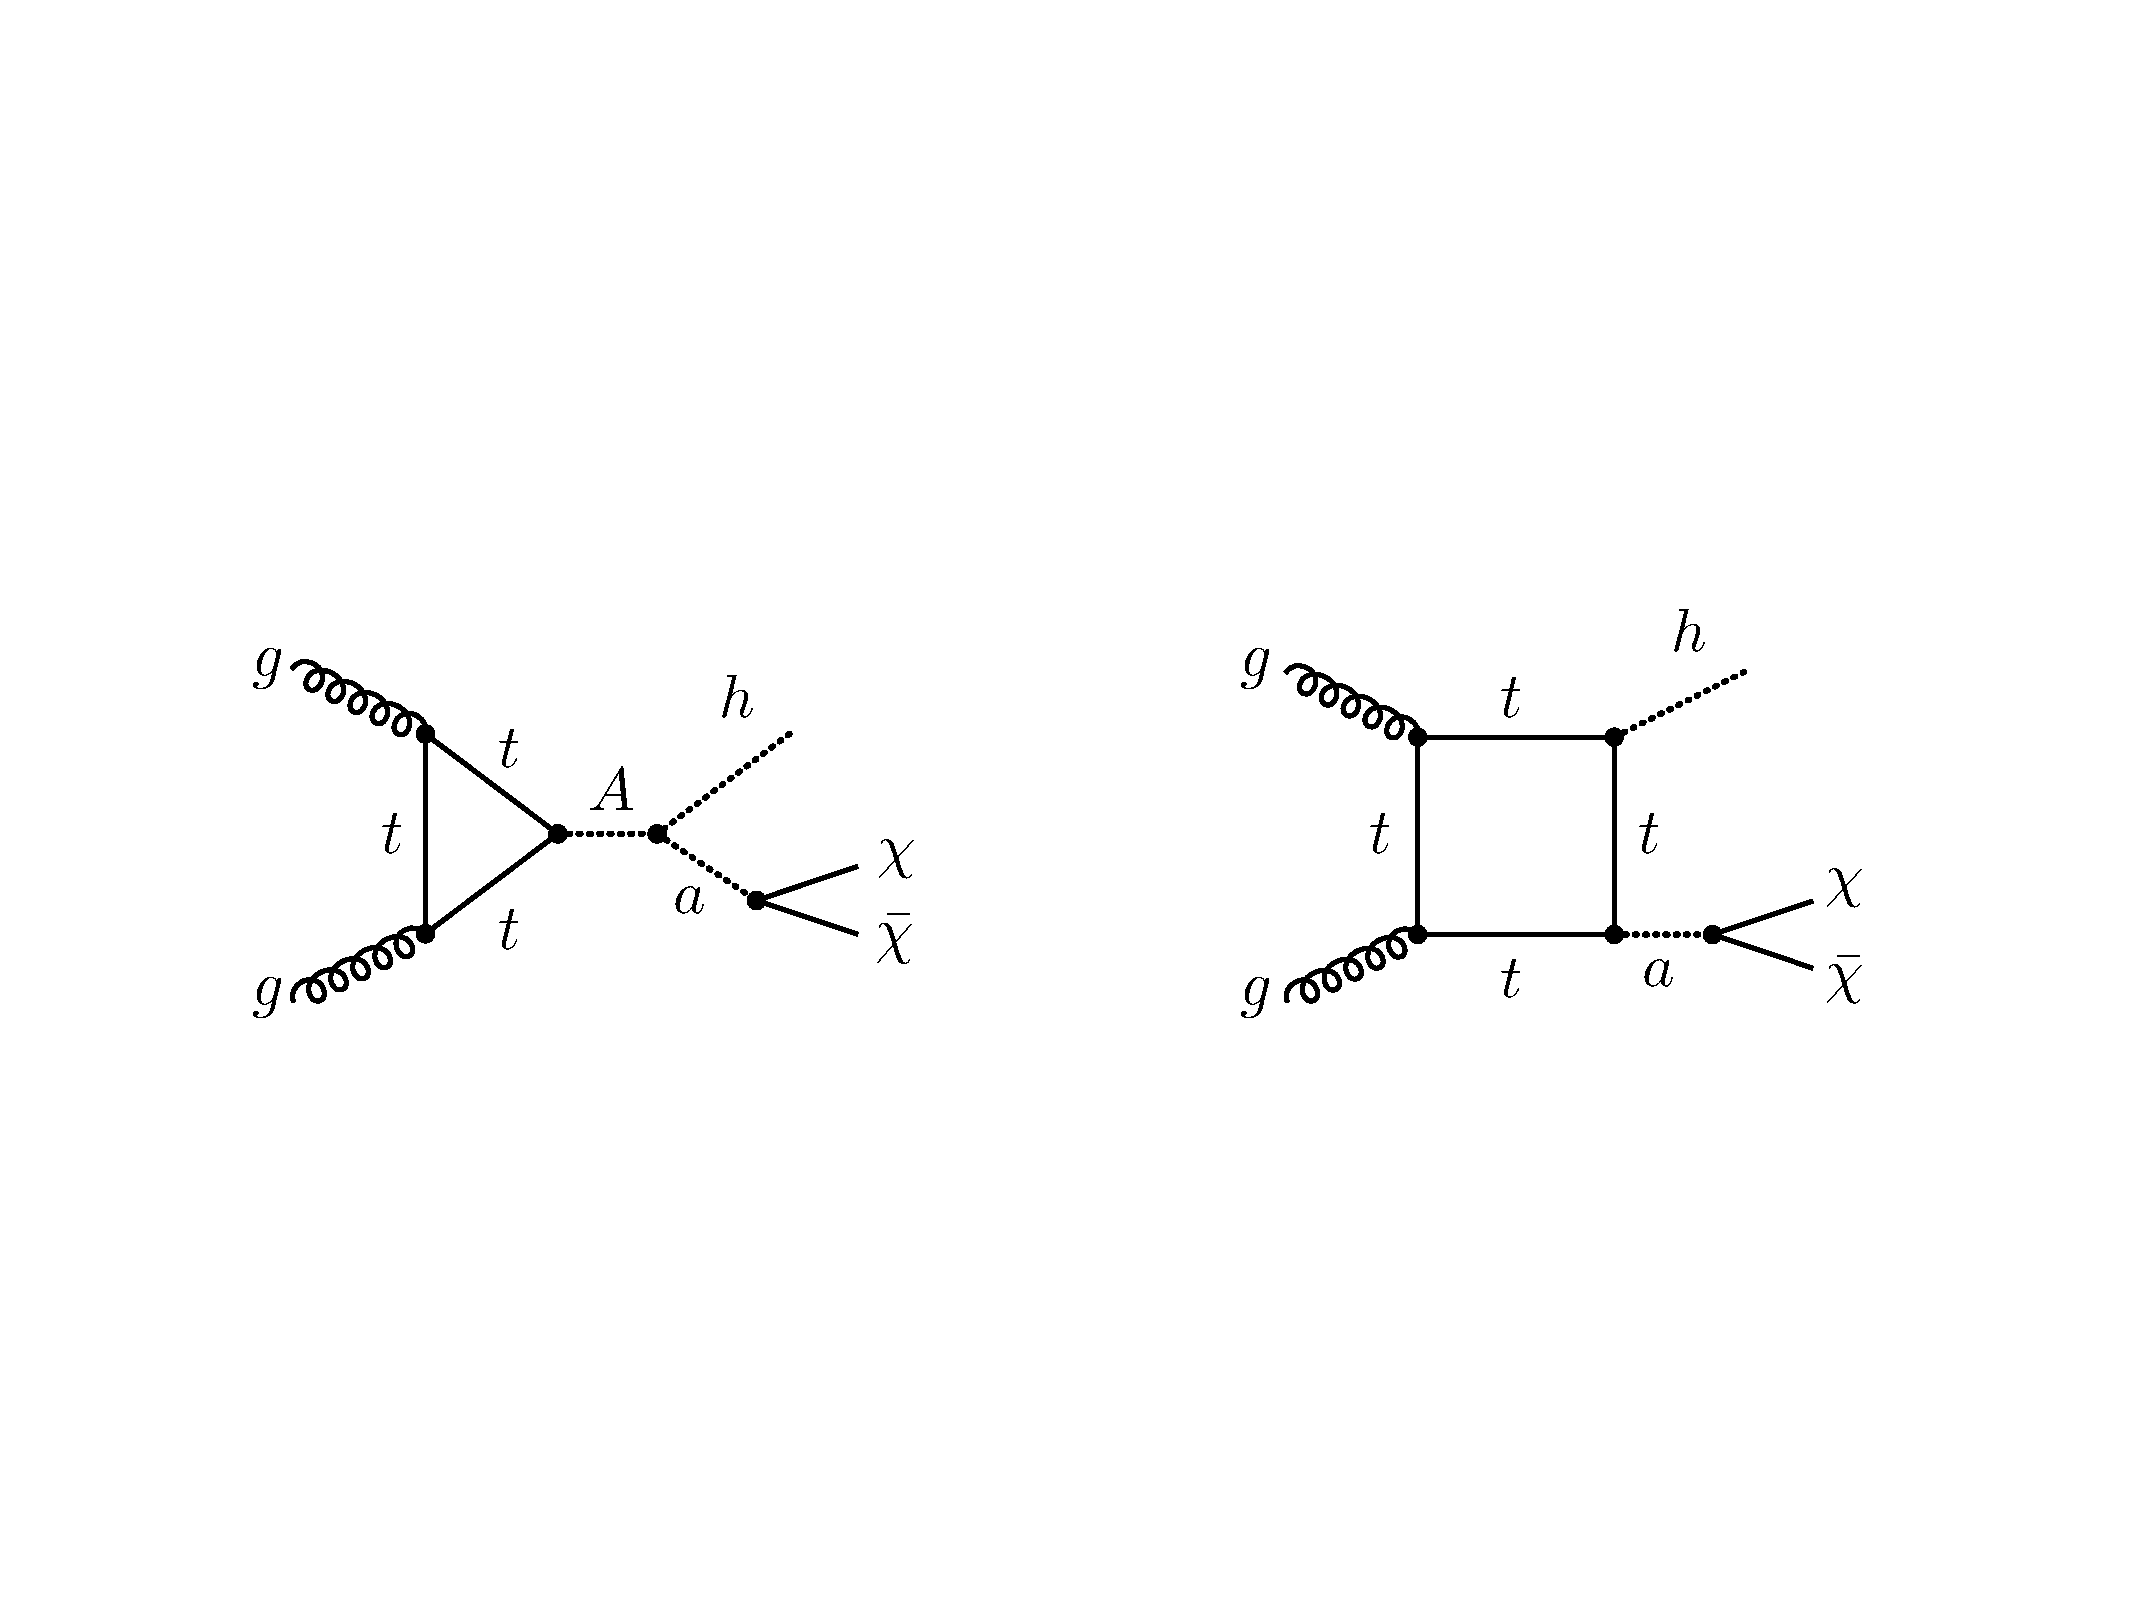
\includegraphics[width=.8\textwidth]{texinputs/04_grid/newfigures/hmet.pdf}

\vspace{4mm}

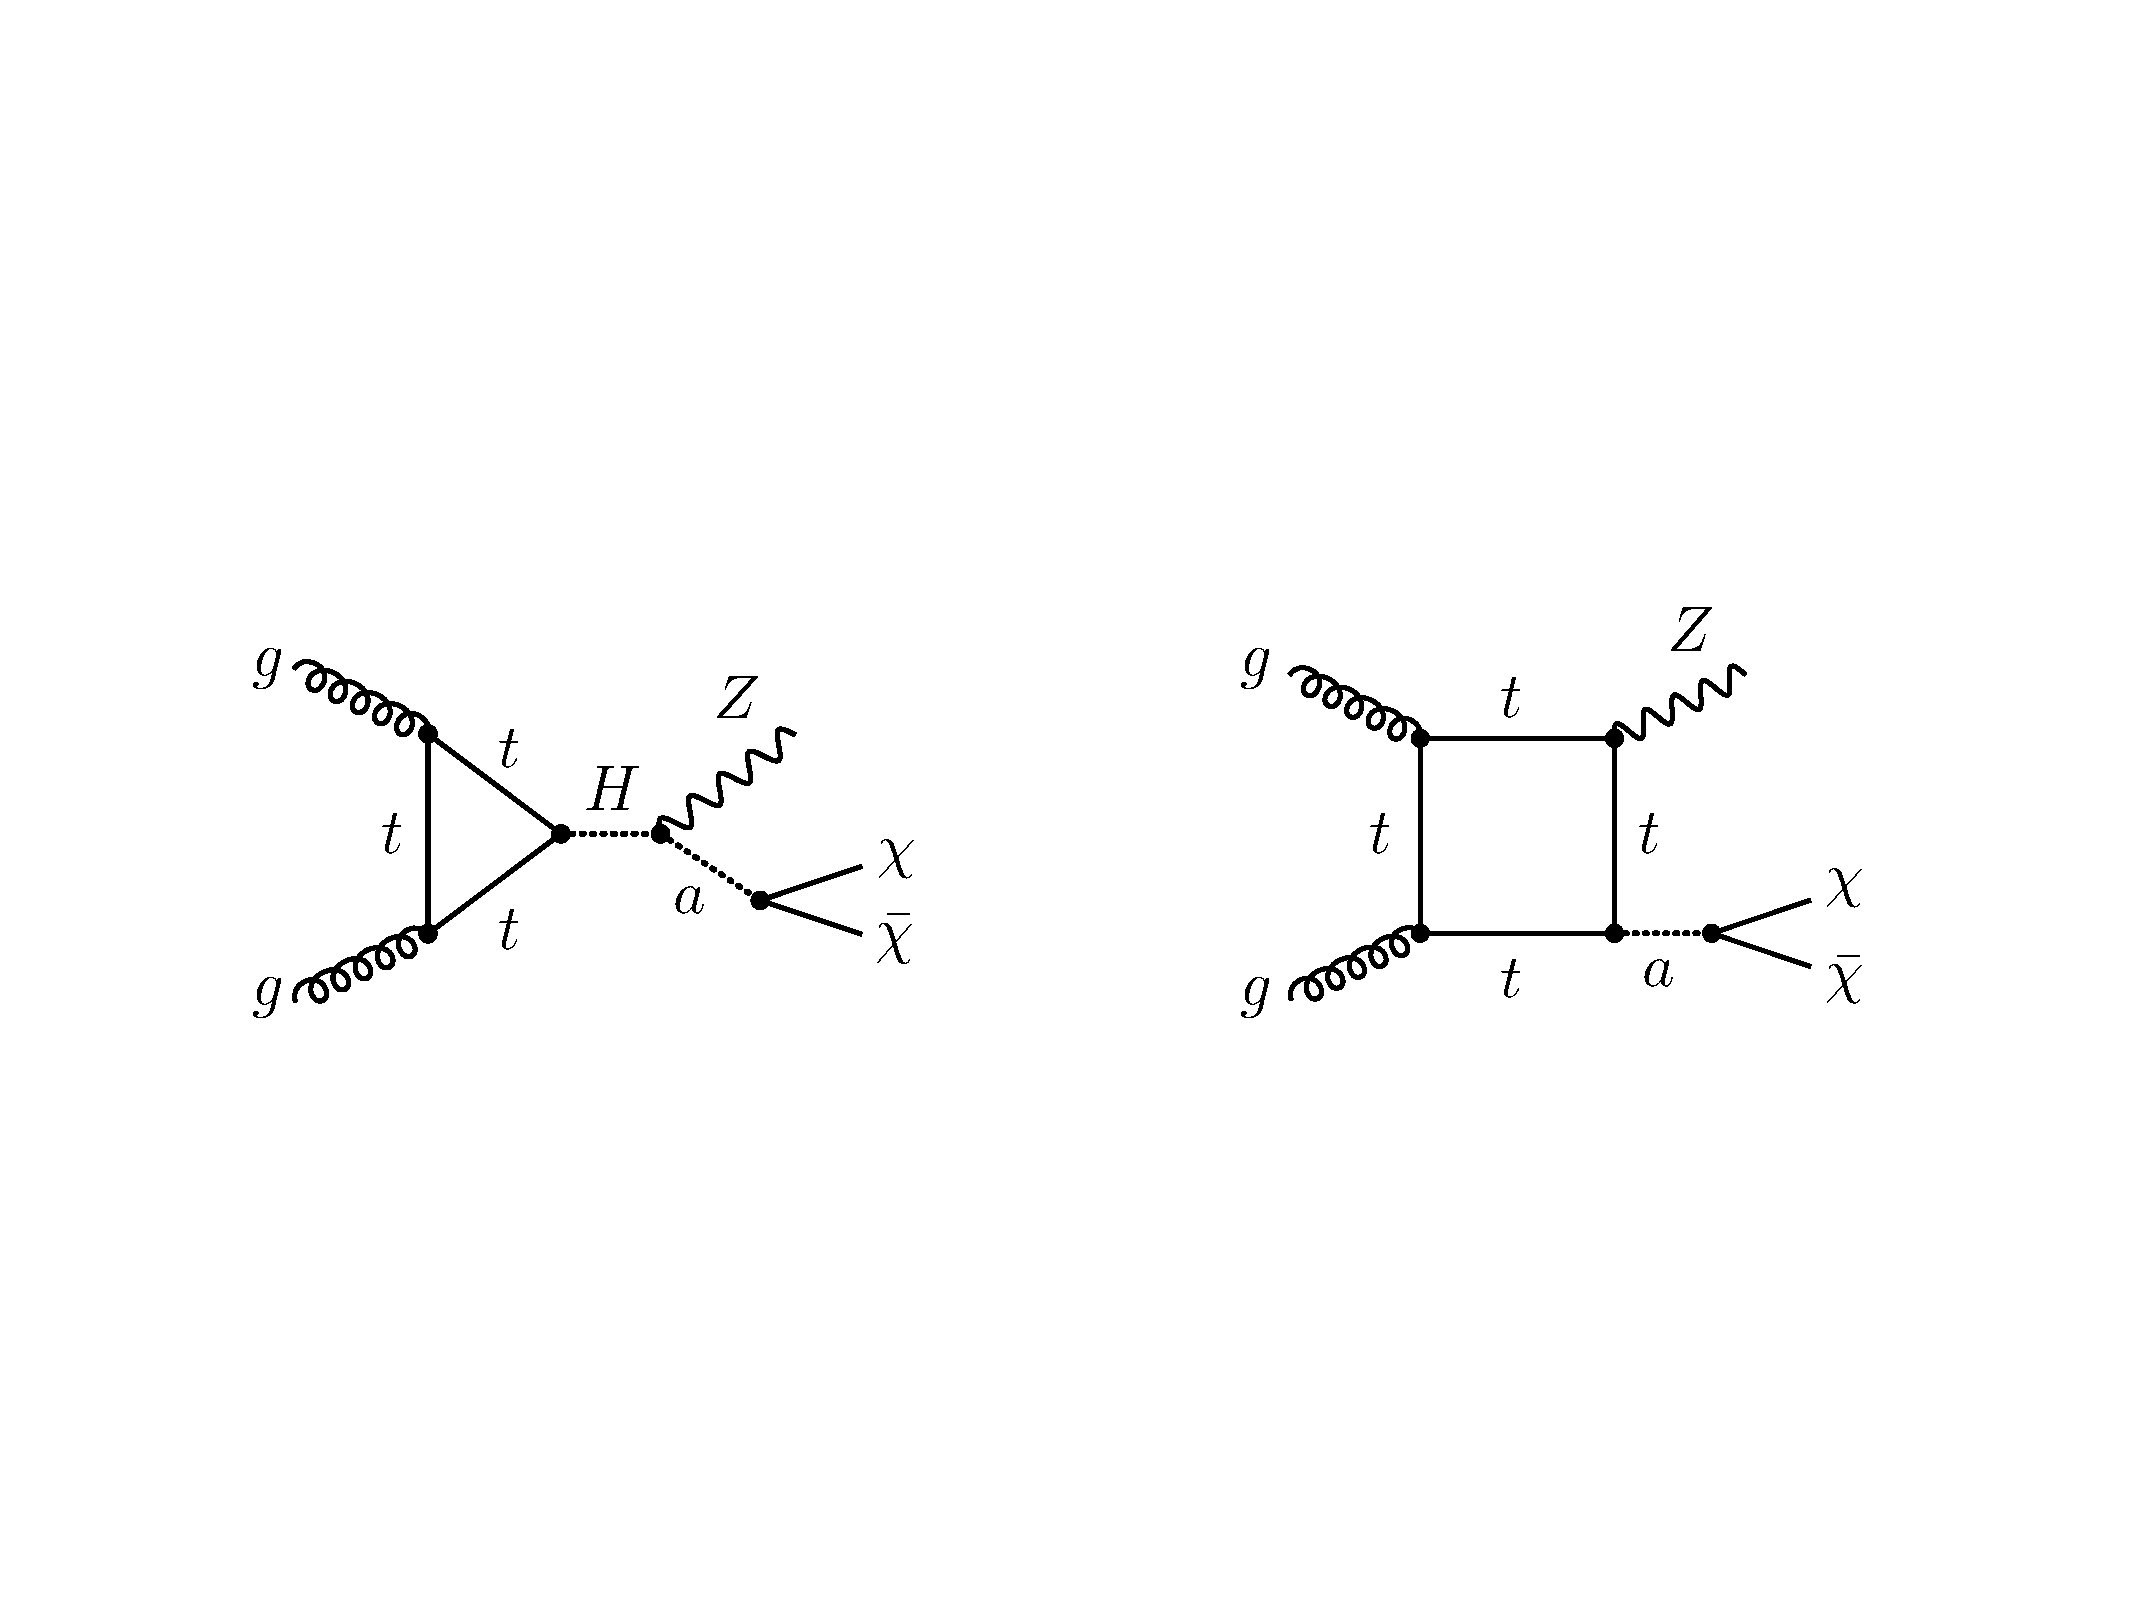
\includegraphics[width=.8\textwidth]{texinputs/04_grid/newfigures/zmet.pdf}

\vspace{5mm}

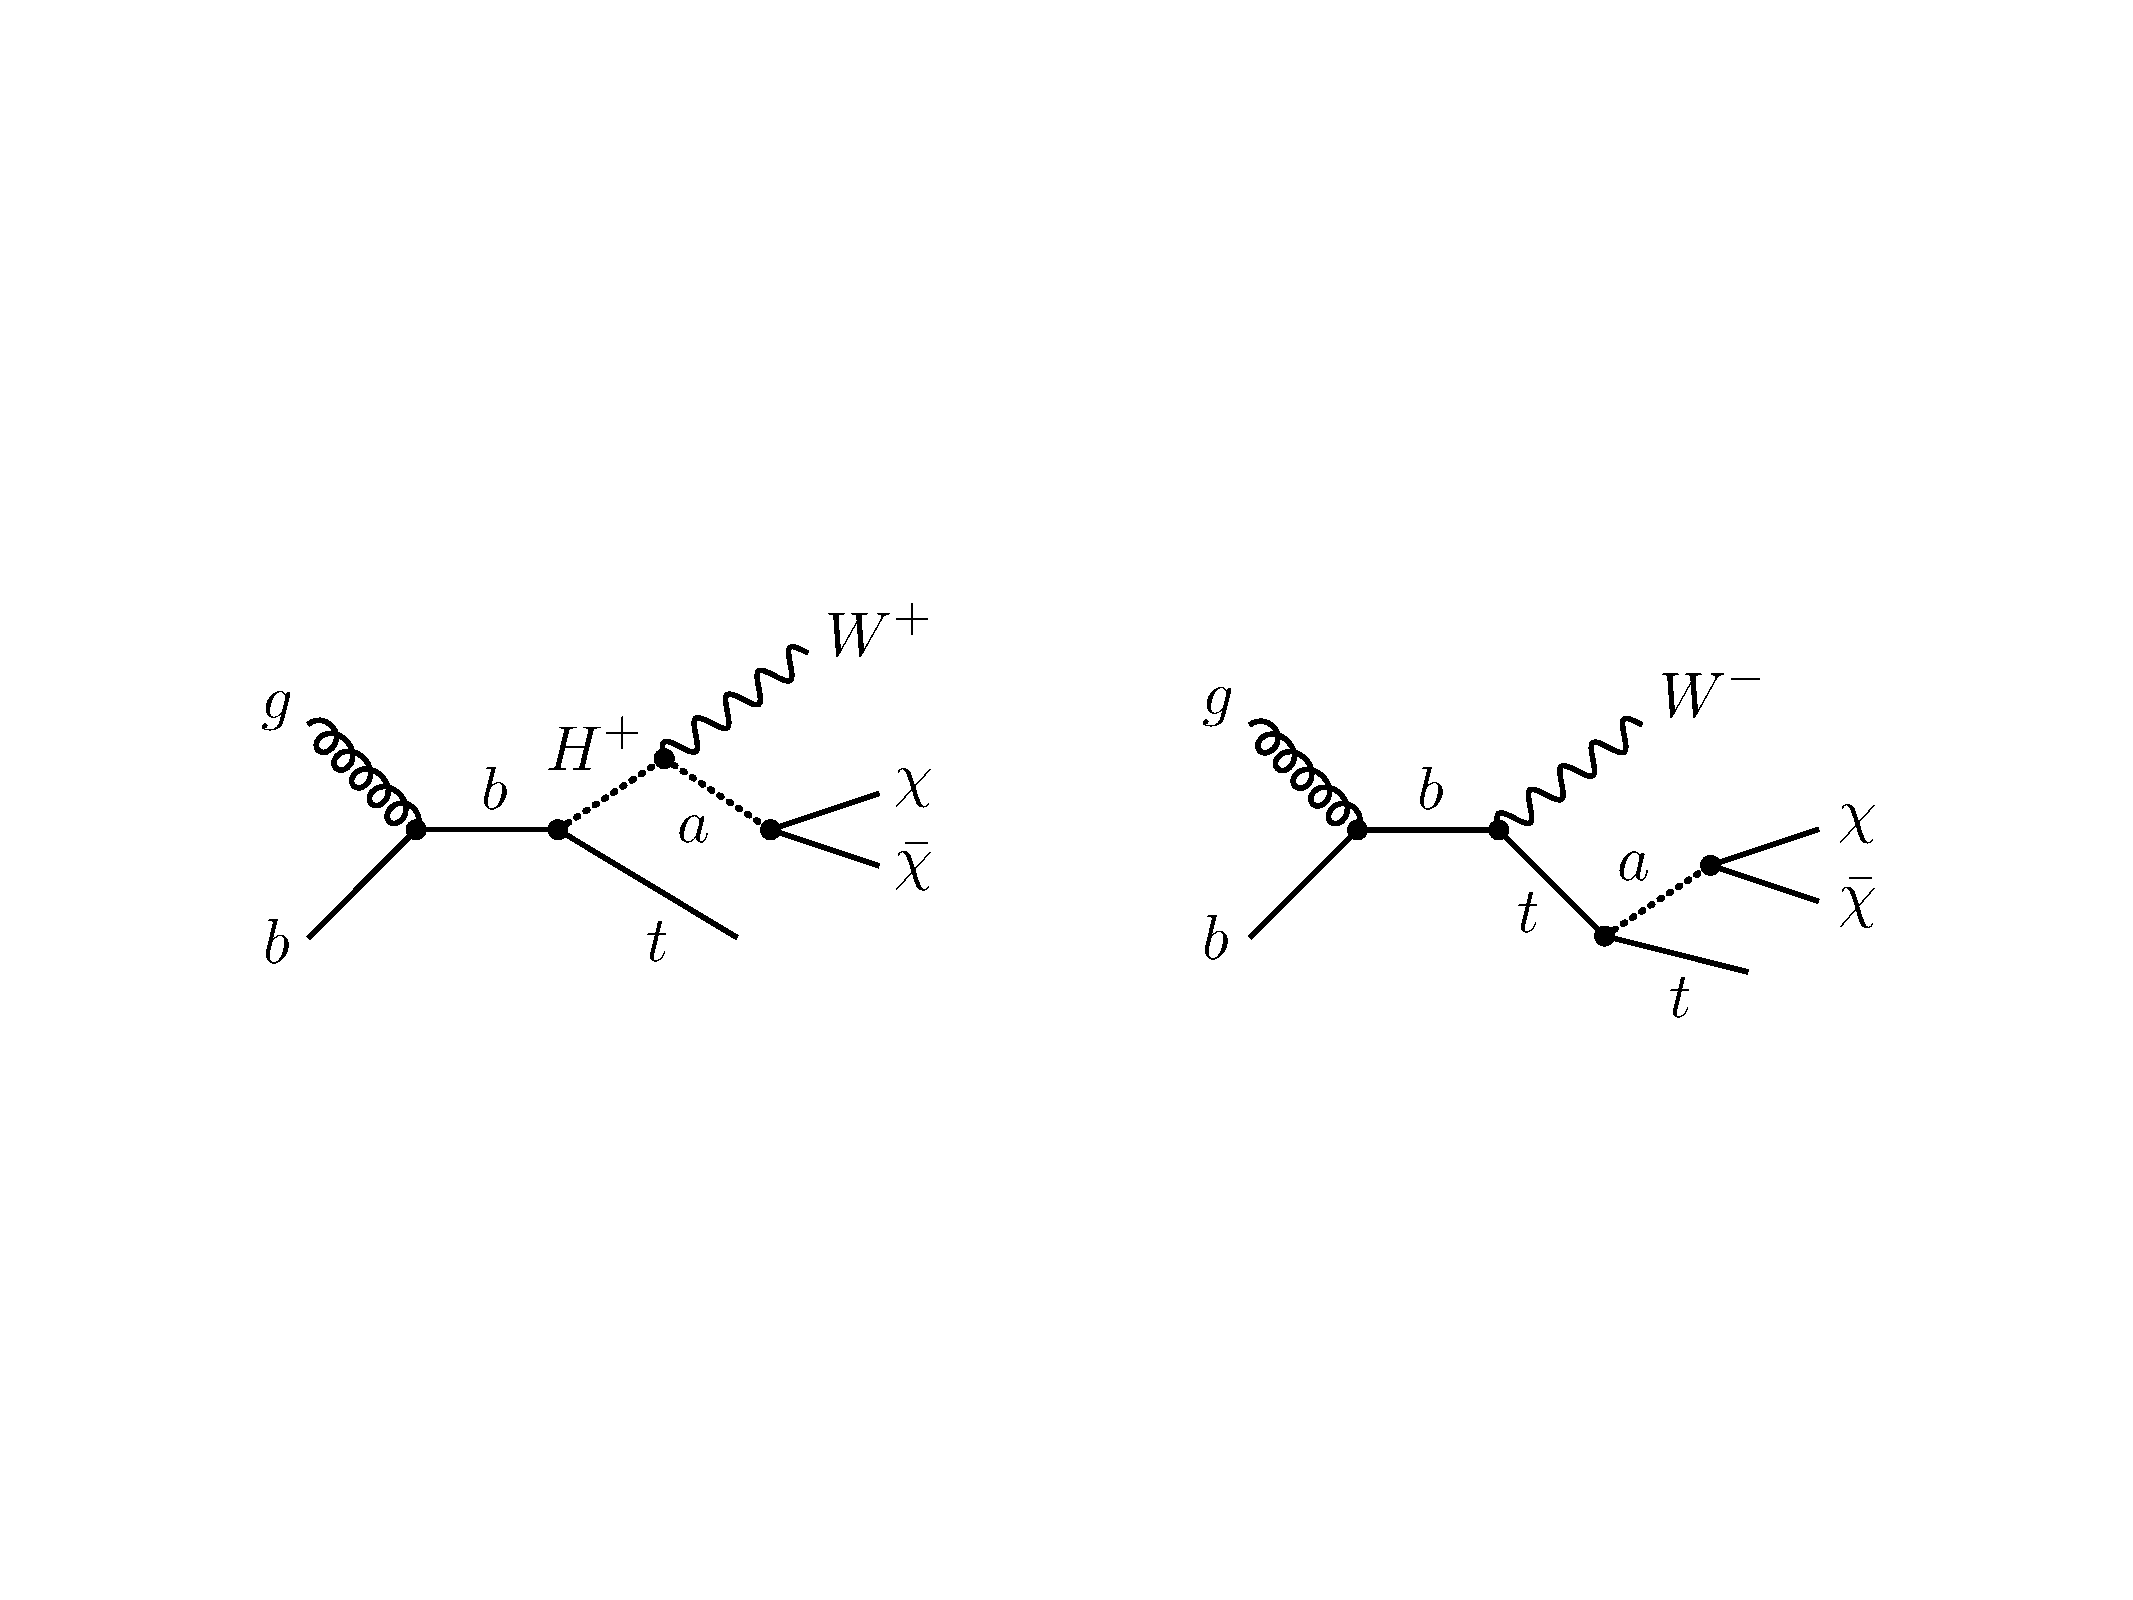
\includegraphics[width=.8\textwidth]{texinputs/04_grid/newfigures/twmet.pdf}

\vspace{4mm}
\caption{\label{fig:resonant} Example diagrams that give rise to a $h+\MET$~(upper row), $Z+\MET$~(middle row) and $tW + \MET$ (lower row) signal in the \hdma model. For further details consult the main text. }
\end{figure}

In the   \hdma model there are broadly speaking two different kinds of $\MET$ signatures. Signals of the first type can be resonantly produced and  channels such as $h+\MET$, $Z+ \MET$ and $tW+\MET$ belong to this class. Relevant examples of Feynman graphs are shown in~Figure~\ref{fig:resonant}. In the case of the mono-Higgs signature, it is evident from the figure that for $M_A > M_h + M_a$ the triangle  graph depicted on the left in the upper row  allows for resonant mono-Higgs production.  Similar resonance enhancements arise from the diagram on the left-hand side for the mono-$Z$ (middle row) and $tW+\MET$ (lower row) channel if $M_H > M_Z + M_a$ and $M_H^\pm > M_W + M_a$, respectively. Notice that resonant $h+\MET$, $Z+\MET$ and $tW+\MET$ production is not possible in the spin-0  DM models proposed by the DM forum (DMF)~\cite{Abercrombie:2015wmb} because in these models the mediators couple only to fermions at tree level. As a result only diagrams of the type shown on the right-hand side of the latter figure are present in  these models. 

\subsection*{Mono-Higgs signature}

\begin{figure}[t!]
\centering
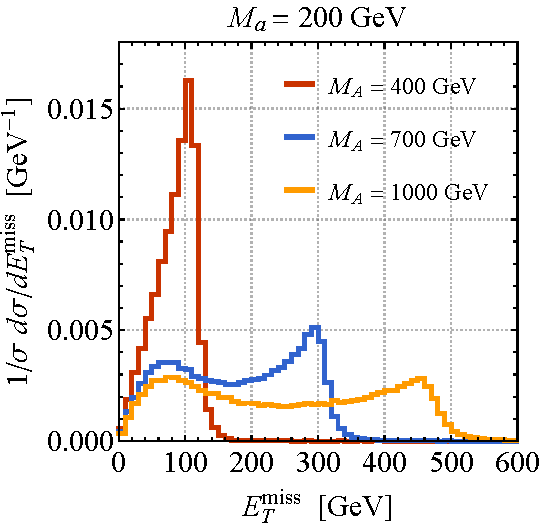
\includegraphics[height=0.45\textwidth]{texinputs/04_grid/newfigures/hmetspecl.pdf}	\qquad 
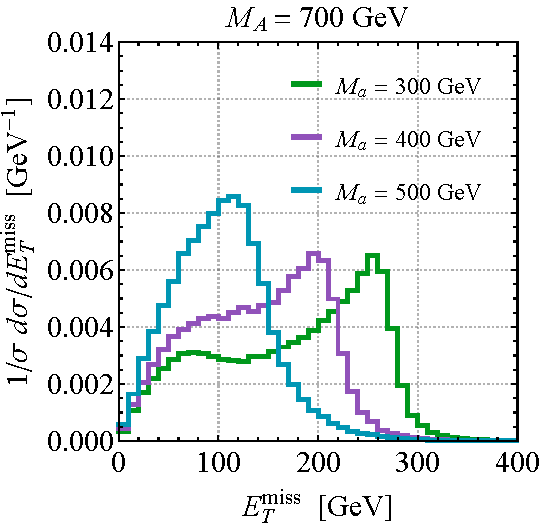
\includegraphics[height=0.45\textwidth]{texinputs/04_grid/newfigures/hmetspecr.pdf}
\vspace{2mm}
\caption{\label{fig:hMET} Normalised $\MET$ distributions of mono-Higgs production in the \hdma model for different values of $\mA$ and $\ma$ as indicated in the legends. The shown results correspond to the benchmark parameter choices introduced in~\eqref{eq:benchmark}. }  
\end{figure}

Processes that are resonantly enhanced in the \hdma model have in common that they involve the on-shell decay of a heavy Higgs $H,A,H^\pm$ to a SM particle and the mediator~$a$, which   itself  subsequently decays to a pair of DM particles. The kinematics of the process $A \to B C$ is governed by the two-body phase space for three massive particles 
\begin{equation} \label{eq:twophasespace}
\lambda(m_A, m_B, m_C) = (m_A^2 -m_B^2-m_C^2)^2 -  4 \hspace{0.25mm} m_B^2 \hspace{0.25mm}  m_C^2 \,,
\end{equation}
and this quantity determines the characteristic shape of resonant $\MET$ signals in the context of the \hdma model. For instance, in the case of the mono-Higgs signal the $\MET$ spectrum  will have a Jacobian peak with an endpoint at~\cite{No:2015xqa,Bauer:2017ota}
\begin{equation} \label{eq:monoHMETpeak}
E^{\rm{miss}}_{T, {\rm max} } \simeq \frac{\lambda^{1/2}(M_A, M_h, M_a)}{2 M_A^2}\,, 
\end{equation}
for all mass configurations that satisfy $M_A > M_h + M_a$. 

In Figure~\ref{fig:hMET} we show the predictions for the normalised $\MET$ distribution of $h+\MET$ production in the \hdma model for different Higgs masses $\mA$ and $\ma$. Besides the indicated values of $\mA$ and $\ma$ the parameters  used  are those given in~\eqref{eq:benchmark}. As can be seen from the figure,  increasing~$\mA$ ($\ma$) shifts the endpoint of the Jacobian peak to higher~(lower) $\MET$  values as expected from~\eqref{eq:monoHMETpeak}. A~second feature that is also visible is  the plot is that for large mass splittings~$\mA - \ma$, the $\MET$ spectra develop a pronounced low-$\MET$ tail. The events in these tails arise dominantly from the box diagram shown on the right in the upper row of~Figure~\ref{fig:resonant}. One can also see that these non-resonant contributions interfere with the resonant contributions that stem from triangle graphs. Due to the interplay of resonant and non-resonant contributions  the exact shape of the $\MET$ distribution is   away from the endpoint~\eqref{eq:monoHMETpeak} a non-trivial function of the \hdma parameters~\eqref{eq:inputparameters}.  

At the LHC a mono-Higgs signal has so far been searched for in the $h \to \gamma \gamma$ and the~$h \to b \bar b$ channel (see~\cite{Aaboud:2017uak,Aaboud:2017yqz,CMS-PAS-B2G-17-004}  for the latest ATLAS and CMS results).  While both searches use $\MET$ as the main selection variable to discriminate signal from background, the $\MET$ values for which the $\gamma \gamma + \MET$ search is most sensitive are smaller than those that give the highest sensitivity in the case of $b \bar b + \MET$. This feature makes the two modes complementary in the sense that a models with  small  splittings $\mA - \ma$ are best probed in the former channel, while realisations with a larger mass hierarchy can be well tested via the latter final state. The decay channel~$h \to WW$ also offers interesting prospects to search for a mono-Higgs signal in the \hdma model~\cite{GPHeidelberg} but as yet has not been studied by the LHC collaborations.  Auxiliary figures showing mono-Higgs distributions in the \hdma model can be found in Appendix~\ref{app:extramonoh}. 

\subsection*{Mono-$\bm{Z}$ signature}

\begin{figure}[t!]
\centering
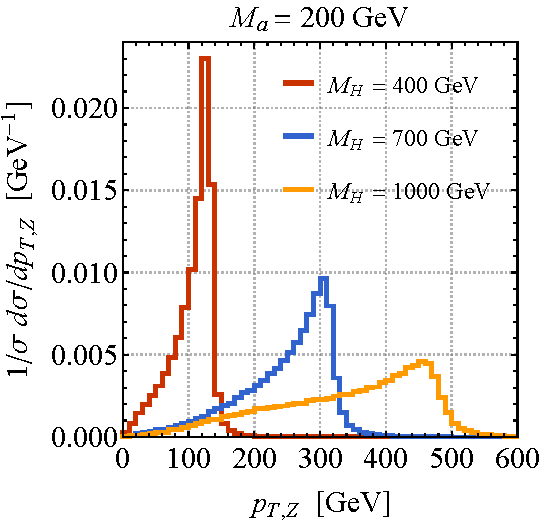
\includegraphics[height=0.45\textwidth]{texinputs/04_grid/newfigures/ptzspec.pdf}	\qquad 
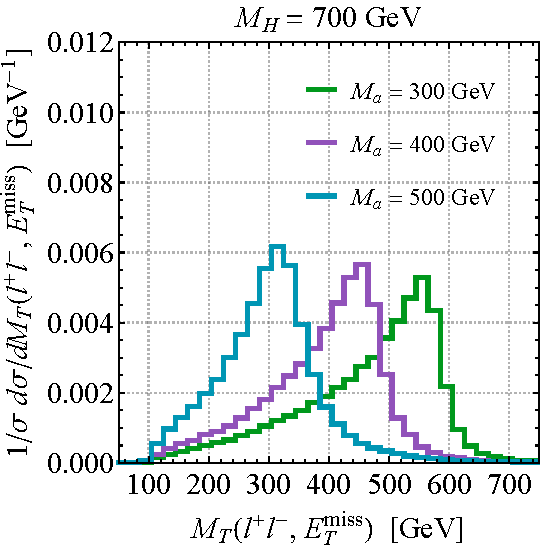
\includegraphics[height=0.45\textwidth]{texinputs/04_grid/newfigures/mtspec.pdf}
\vspace{2mm}
\caption{\label{fig:zptmt} Normalised $p_{T,Z}$ (left panel) and $M_T (\ell^+ \ell^-, \MET)$ (right panel) distributions for $Z + \MET$ production followed by $Z \to \ell^+ \ell^-$. The shown predictions have been obtained for the \hdma benchmark parameter choices  given in~\eqref{eq:benchmark} and employ different values of~$M_H$ and~$M_a$ as indicated in the legends.}
\end{figure}

Like for the mono-Higgs signal also in the mono-$Z$ case shape analyses of the~$\MET$ variable offer a powerful way to enhance the signal-to-backround ratio. The endpoint of the $\MET$ spectrum for the $Z+\MET$ signature can be simply obtained from~\eqref{eq:monoHMETpeak} by the replacements $M_A \to M_H$ and $M_h \to M_Z$. Plots that show the corresponding $\MET$ distributions are relegated to Appendix~\ref{app:extramonoz}. Since the four-momenta of the decay products $Z$ and $a$ that enter $H \to Za$ are fixed by $H$ being preferentially on-shell, also the spectrum of the $Z$-boson transverse momentum ($p_{T,Z}$) in mono-$Z$ production will have a characteristic shape if $M_H > M_Z + M_a$. In fact,  the $p_{T,Z}$ distribution is like the $\MET$ spectrum predicted  to be Jacobian with a cut-off at~\cite{No:2015xqa,Bauer:2017ota}
\begin{equation} \label{eq:monoZpTpeak}
p_{T,Z}^{ {\rm max} } \simeq \frac{\lambda^{1/2}(M_H, M_Z, M_a)}{2 M_H^2}\,,
\end{equation}
that is smeared by the total decay width $\Gamma_H$ of the heavy Higgs $H$. Notice that  ignoring parton-shower and detector effects the shapes of the $p_{T,Z}$ and $\MET$ spectra are identical. Whether a shape fit to $\MET$ or $p_{T,Z}$ provides a better experimental reach thus depends to first approximation only on which of the two variables can be better measured.

Another useful observable to study the properties of processes involving visible and invisible decay production is the transverse mass 
\begin{equation} \label{eq:transversemass}
M_T (A,B) = \sqrt{m_A^2+m_B^2 + 2 \left (E_{T,A} E_{T,B} - \vec{p}_{T,A} \cdot \vec{p}_{T,B} \right )} \,,
\end{equation}
where $E_{T,A}$ ($E_{T,B}$) denotes the transverse energy of the final-state configuration $A$ ($B$) and~$\vec{p}_{T,A}$  ($\vec{p}_{T,B}$) is the corresponding transverse momentum three-vector. In the case of the mono-$Z$ search that looks for the leptonic decay of the $Z$ boson, the transverse mass can be constructed from the $\ell^+ \ell^-$ system and the amount of $\MET$.  

Figure~\ref{fig:zptmt} displays  $p_{T,Z}$ and $M_T(\ell^+ \ell^-, \MET)$ distributions for different choices of the masses~$M_H$ and~$M_a$. The parameters not explicitly specified in the plots have been  fixed to the values reported in~\eqref{eq:benchmark}. One observes that the differential distributions in $p_{T,Z}$ and $M_T(\ell^+ \ell^-, \MET)$ have Jacobian peaks, a feature that  reflects the resonant production of a~$H$ with the subsequent decay $H \to Z a \to \ell^+ \ell^- \chi \bar \chi$.  Increasing~$\mH$ ($\ma$) again shifts the endpoints of the distributions to higher~(lower) values of $p_{T,Z}$ and $M_T(\ell^+ \ell^-, \MET)$. Like in the mono-Higgs case, for large mass differences $M_H - M_a$, box diagrams lead to a non-negligible mono-$Z$ rate at low values of $p_{T,Z}$ and $M_T(\ell^+ \ell^-, \MET)$. Compared to the $h + \MET$ signature the interference effects between resonant and non-resonant contributions  are however  less pronounced  in  the $Z + \MET$  case. Plots showing additional  mono-$Z$ distributions are provided in~Appendix~\ref{app:extramonoz}. 

The existing LHC searches for a mono-$Z$ signal (cf.~\cite{Aaboud:2017bja,Sirunyan:2017qfc} for the most recent results) have  focused either on invisible decays of the SM-like Higgs boson or on topologies where the $Z$~boson is produced in the form of initial-state radiation (ISR). Since ISR of a $Z$~boson is compared to the radiation of a gluon suppressed by both the coupling of the~$Z$ and its mass, the mono-$Z$ signal is generically not a discovery channel in models that lead to ISR-like mono-$X$ signatures. In contrast, in the \hdma model the $Z+\MET$ sensitivity  turns out to be typically better than the one of the mono-jet channel. 

The above discussion has focused on the leptonic decay of the~$Z$~boson but searching for a mono-$Z$ signal in the hadronic channel is also possible. In fact, the hadronic and leptonic signatures  are complementary, since hadronic decays of the~$Z$~boson are more frequent than leptonic decays, but suffer from larger backgrounds. An improved background suppression is possible if ``boosted'' event topologies are studied, making the hadronic mono-$Z$ signature an interesting channel if the \hdma model includes high-mass Higgs states. Further details on $q \bar q + \MET$ search strategies can be found in~Appendix~\ref{app:extramonoz}.

\subsection*{Single-top signatures}

\begin{figure}[t!]
\centering
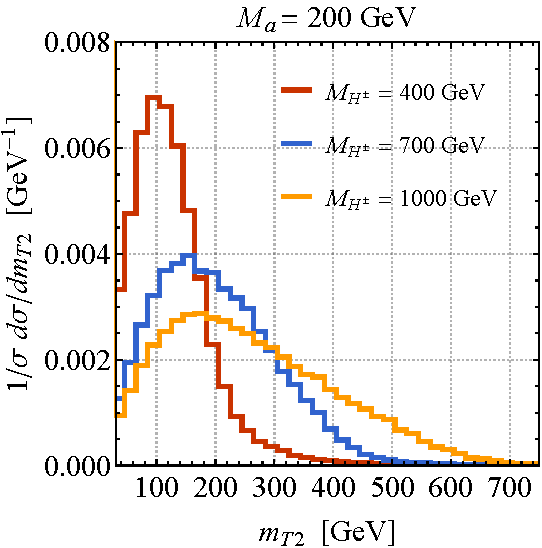
\includegraphics[height=0.45\textwidth]{texinputs/04_grid/newfigures/mt2l.pdf} \qquad 
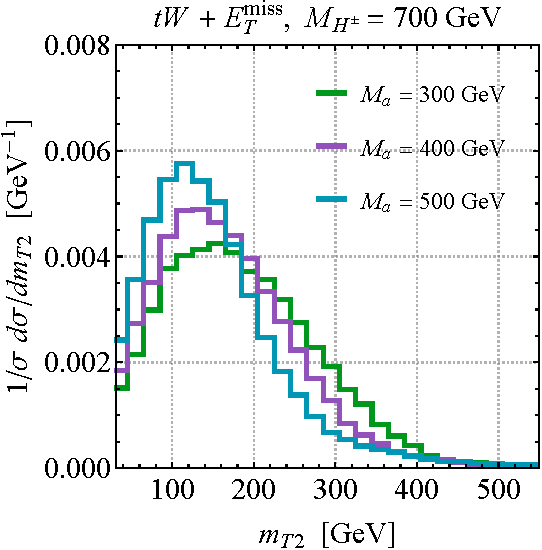
\includegraphics[height=0.45\textwidth]{texinputs/04_grid/newfigures/mt2r.pdf}
\vspace{2mm}
\caption{\label{fig:mt2spectra} Normalised $m_{T2}$ distributions for $tW+\MET$ production in the double-lepton channel.  The shown results correspond to the \hdma benchmark~\eqref{eq:benchmark} and employ different values of~$\mHc$ and~$\ma$ as indicated in the legends.}
\end{figure}

Single-top production in association with $\MET$ has also been shown to be a promising mono-$X$ channel in the case of spin-0 models~\cite{Pinna:2017tay,Pani:2017qyd,Plehn:2017bys}. One can study single-top production in the $s$-channel, $t$-channel  or  in association with a $W$ boson. In the following, we will focus on the $tW + \MET$ channel, which in the context of the \hdma model has been identified as the most interesting mode~\cite{Pani:2017qyd}. Example diagrams leading to a $tW + \MET$ signature are shown in the lower row of~Figure~\ref{fig:resonant}. The $tW + \MET$ signal can be searched for in the single-lepton and double-lepton final state. Analysis strategies for both channels have been developed in~\cite{Pani:2017qyd}. In the former case $M_T (\ell, \MET)$ and the asymmetric transverse mass $am_{T2}$~\cite{Konar:2009qr,Lester:2014yga} can be used to discriminate between signal and background, while in the latter case the stransverse mass $m_{T2}$~\cite{Lester:1999tx,Barr:2003rg} plays a crucial role in the background suppression.

Examples of normalised $m_{T2}$ distributions obtained in the \hdma model are shown in Figure~\ref{fig:mt2spectra}. The coloured histograms correspond to different masses $\mHc$ and $\ma$. The parameters not indicated in the legends have been set to the values given in~\eqref{eq:benchmark}. One sees from the plots that the shape of the $m_{T2}$ spectrum is sensitive to the values that are chosen for $\mHc$ and $\ma$. In particular, the maximum of the $m_{T2}$ distribution is shifted to higher values for larger (smaller) values of $\mHc$ ($\ma$). Notice that for heavy charged Higgses the $m_{T2}$ spectrum develops a pronounced high-$m_{T2}$ tail.  This feature can be traced back to the resonant contribution $b g \to t H^+  \to  t W^+ a  \to t W^+ \chi \bar \chi$ (see~lower left graph in~Figure~\ref{fig:resonant}). At present, dedicated ATLAS and CMS analyses of the $tW + \MET$  or other single-top-like signatures with $\MET$ do not exist. Performing such studies would however be worthwhile since enhanced single-top signatures are expected to appear in many DM model that features an extended Higgs sector. 

\subsection[Non-resonant $E_T^{\rm miss}$ signatures]{Non-resonant $\bm{E_T^{\rm miss}}$ signatures}
\label{sec:nonresonant}

\begin{figure}[t!]
\centering
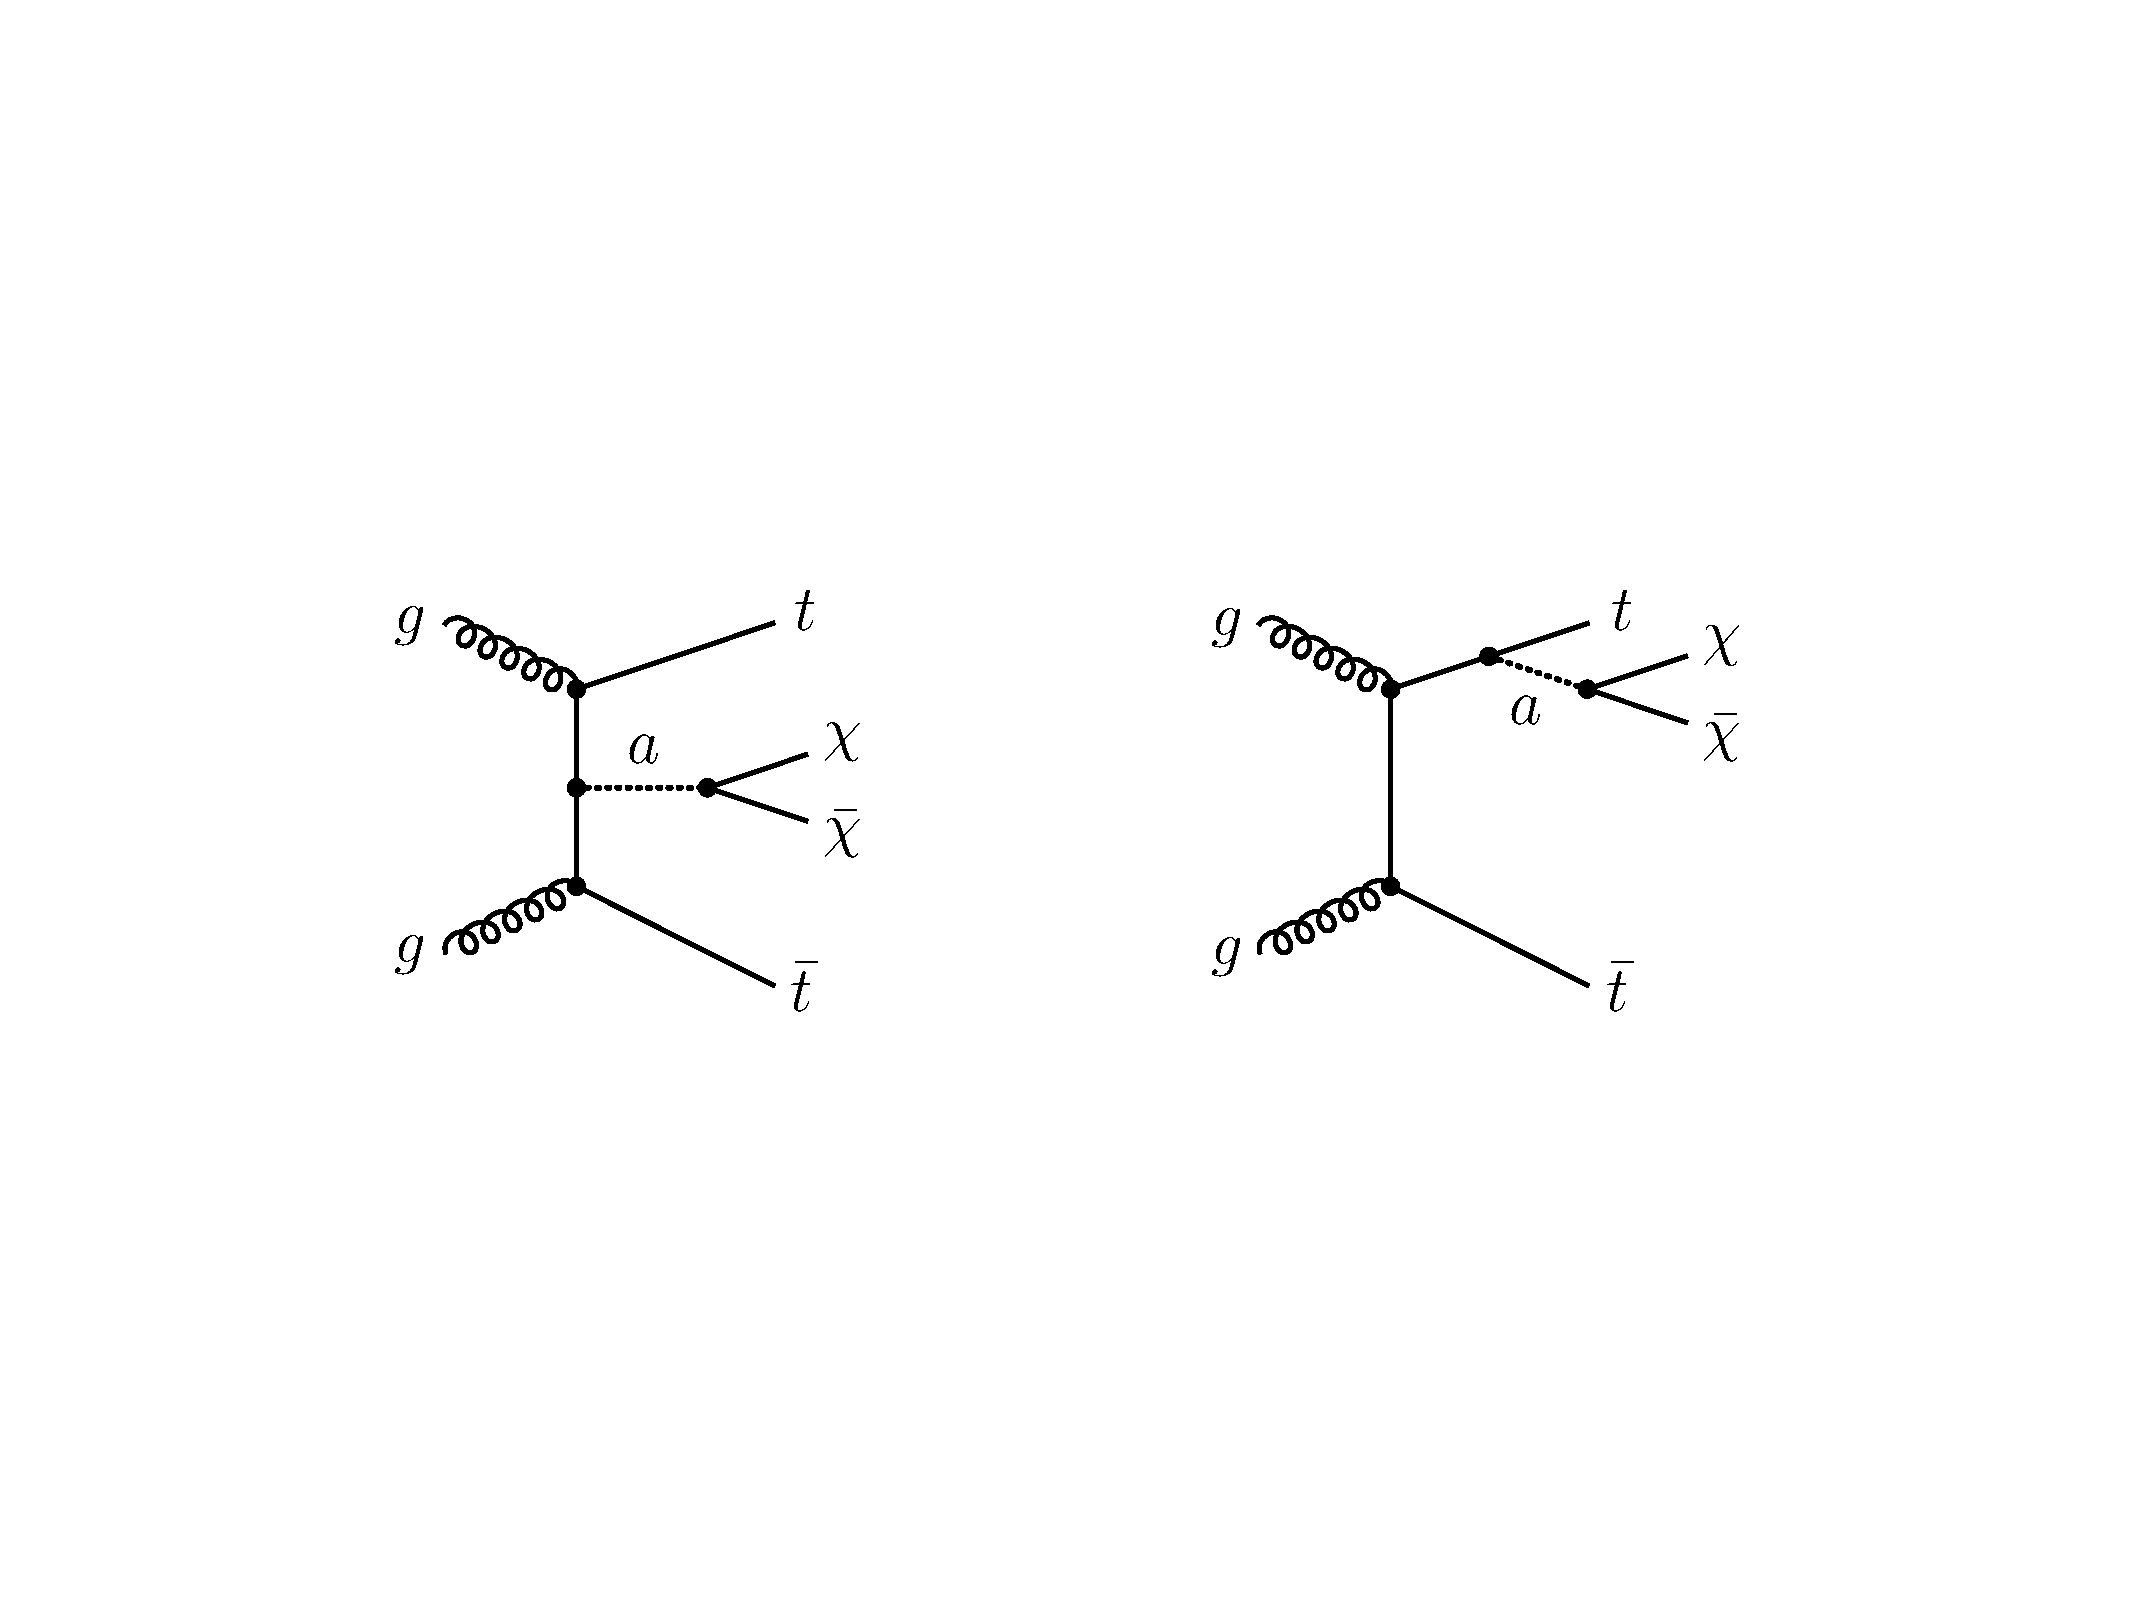
\includegraphics[width=.725\textwidth]{texinputs/04_grid/newfigures/ttmet.pdf}

\vspace{7mm}

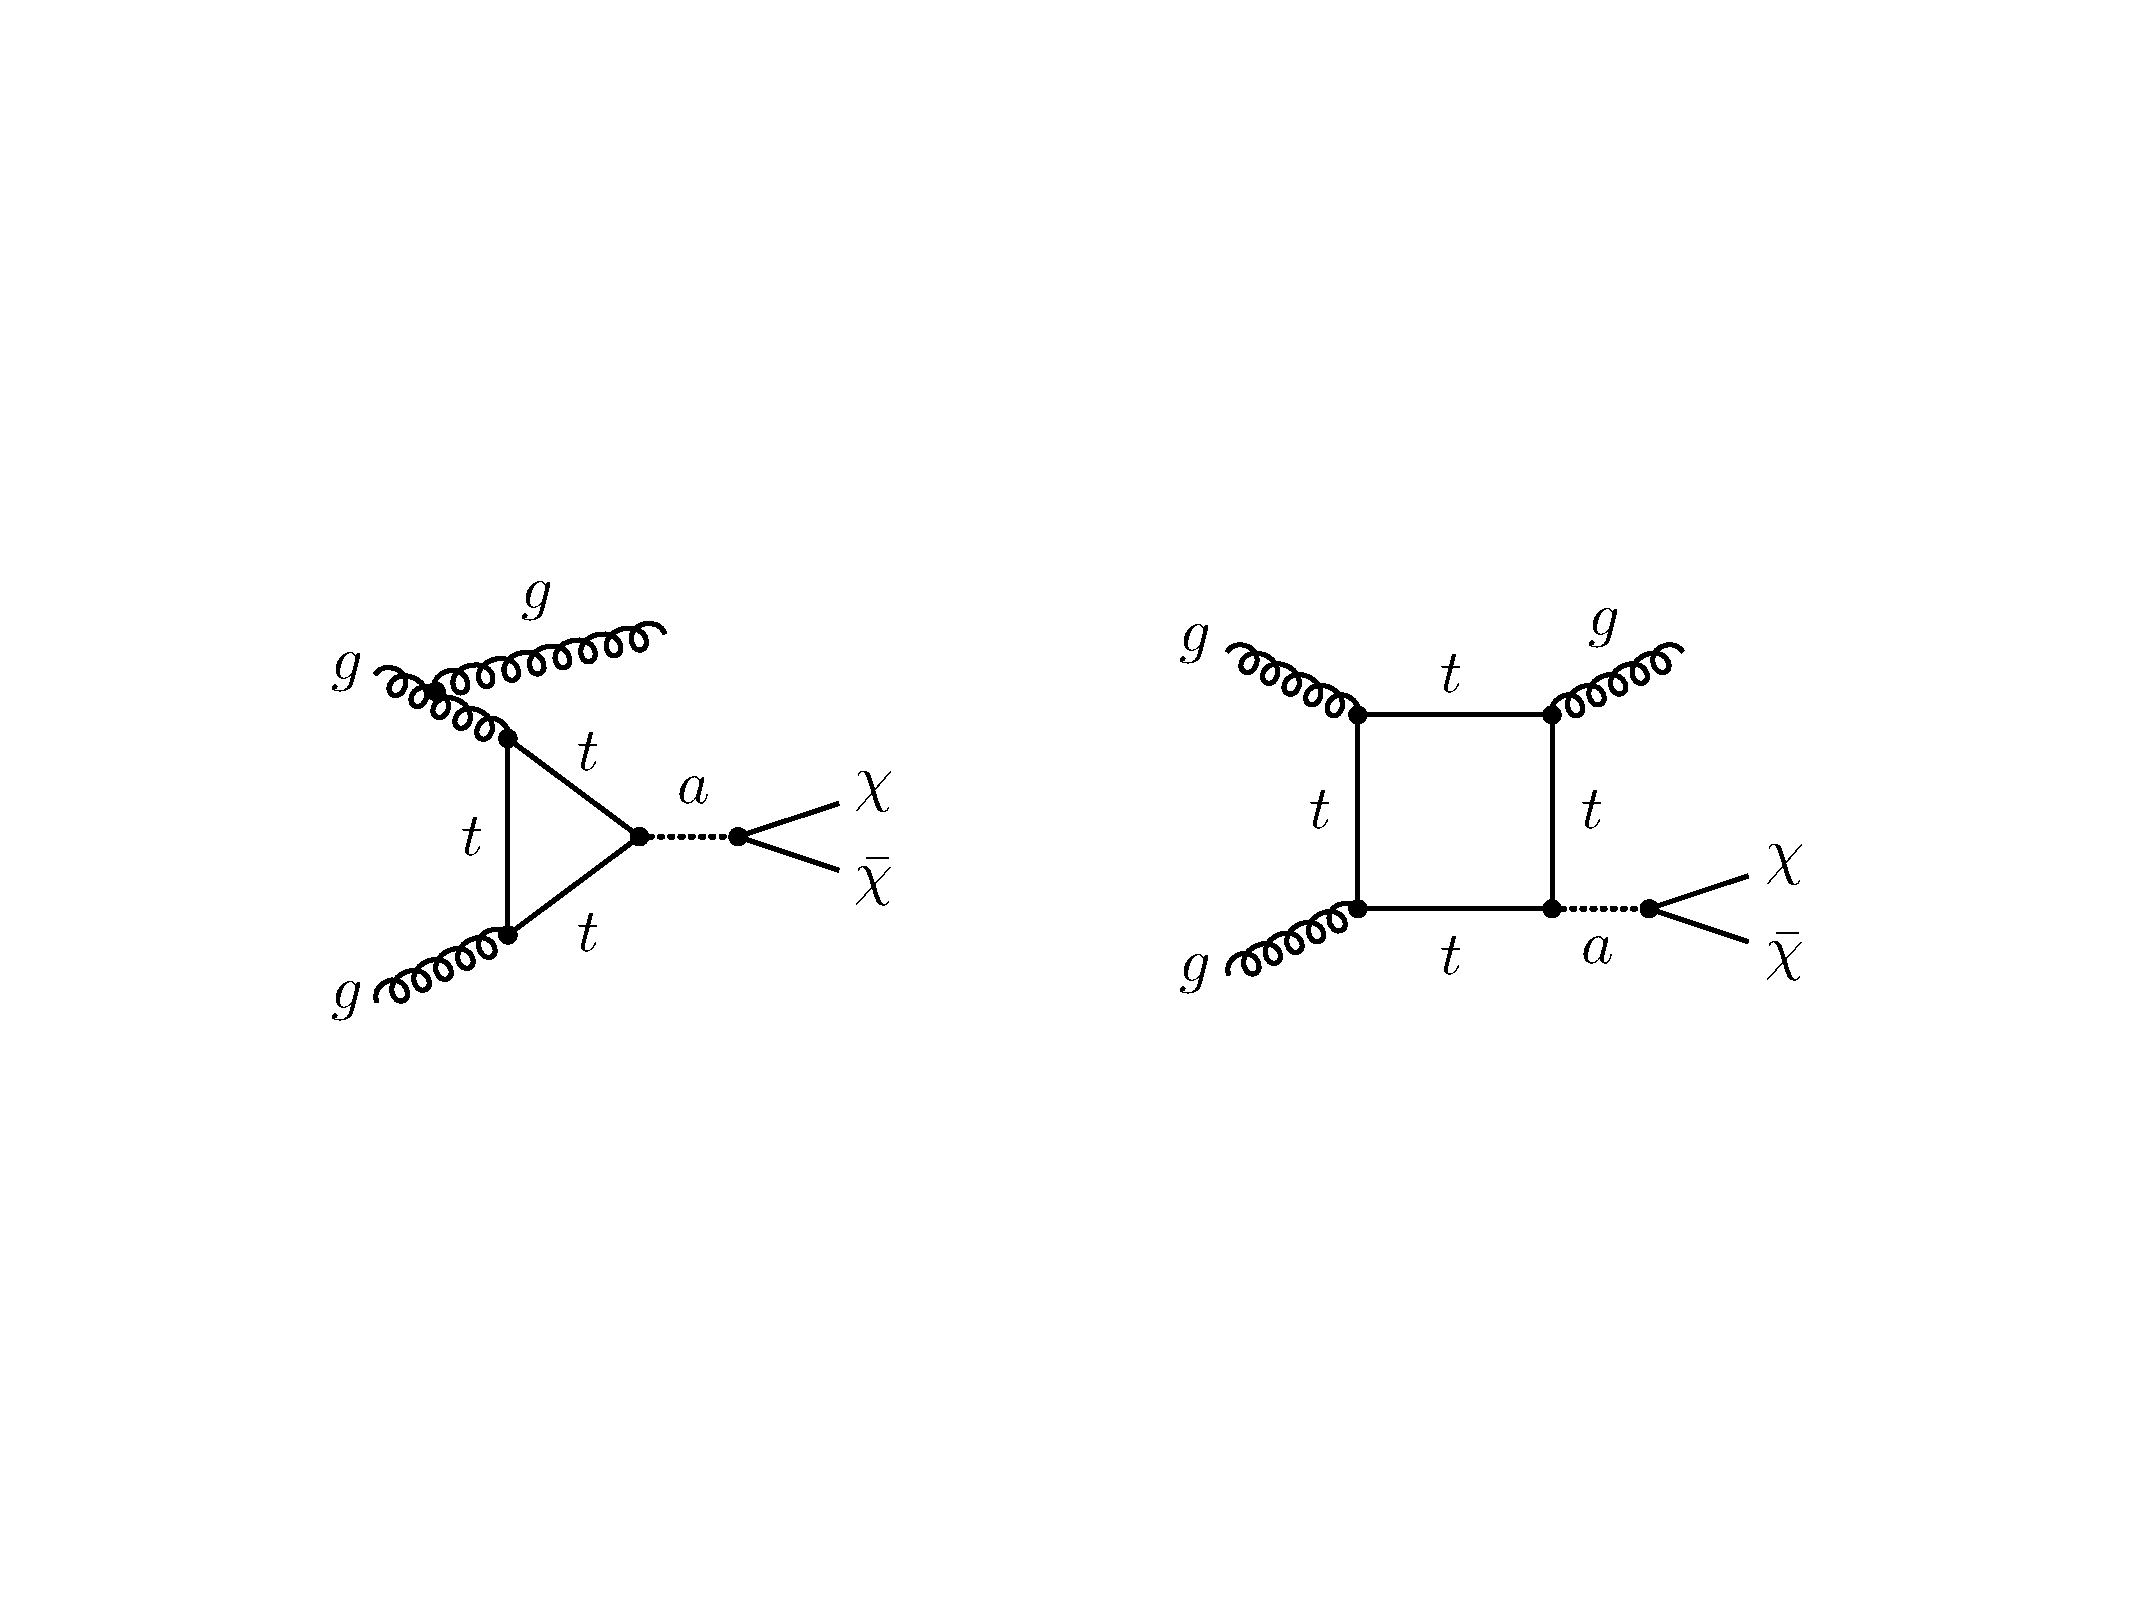
\includegraphics[width=.8\textwidth]{texinputs/04_grid/newfigures/jmet.pdf}

\vspace{4mm}
\caption{\label{fig:nonresonant} Prototype diagrams that lead  to a $t \bar t+\MET$~(upper row) and $j+\MET$~(lower row) signal in the \hdma model. Graphs involving a heavier pseudoscalar $A$ also contribute to the signals but are not shown explicitly.}
\end{figure}

Besides the resonant $\MET$ signatures discussed in the last subsection the   \hdma model also gives rise to non-resonant mono-$X$ signatures. The most important channels in this class are $t \bar t +\MET$ and $j+\MET$ production, but also  the $b \bar b +\MET$ mode is interesting  because its rate is $\tan \beta$ enhanced if a Yukawa sector of  type-II is realised.  Representative Feynman graphs leading to the first two signatures are depicted in~Figure~\ref{fig:nonresonant}. Notice that for $M_A \gg M_a > 2 m_\chi$ the dominant contribution to the  $t \bar t +\MET$ and mono-jet signals arise from graphs involving the  mediator $a$. In this limit the normalised kinematic distributions of the $t \bar t + \MET$ and $j+\MET$ signals in the \hdma model therefore resemble the shapes of the spectra obtained in the DMF pseudoscalar   model. Since the contributions  associated to $a$ and $A$ exchange interfere with each other, shape differences can however occur if the pseudoscalars are not widely separated in mass~\cite{Bauer:2017ota}.

\subsection*{Heavy-quark signatures}

\begin{figure}[t!]
\centering
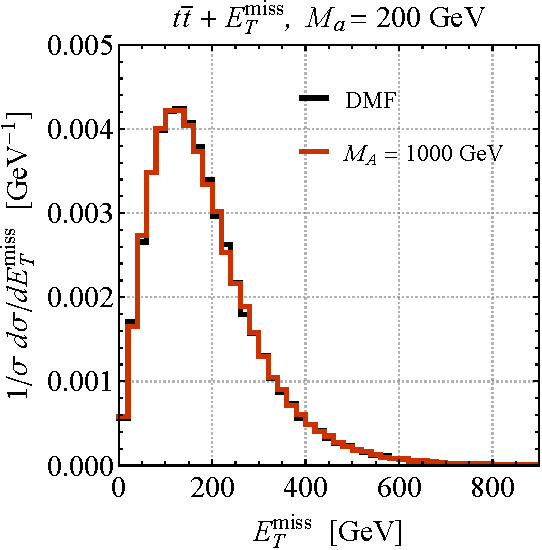
\includegraphics[height=0.45\textwidth]{texinputs/04_grid/newfigures/ttmetl.pdf} \qquad 
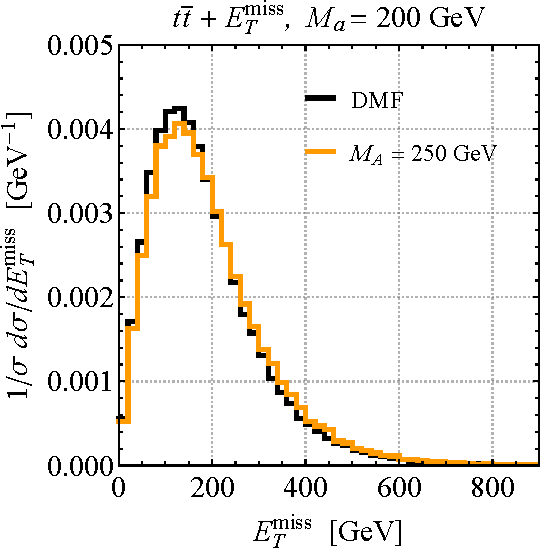
\includegraphics[height=0.45\textwidth]{texinputs/04_grid/newfigures/ttmetr.pdf}
\vspace{2mm}
\caption{\label{fig:ttmet} Normalised $\MET$ distributions for $t \bar t + \MET$ production. The black curves correspond to the prediction of the DMF pseudoscalar   model, while the coloured predictions illustrate the results in the \hdma benchmark model~\eqref{eq:benchmark} for two different choices of $\mA$ and $\ma$.} 
\end{figure}

Two of the main channels that have been used up to now  to search for spin-0 states with large invisible decay widths at the LHC are $t \bar t + \MET$ and $b \bar b + \MET$. The latest ATLAS and CMS analyses of this type can be found in~\cite{Aaboud:2017rzf,CMS-PAS-EXO-16-049}. These searches have been interpreted in the context of the DMF spin-0   models, and for $M_A \gg M_a$ the obtained cross-section limits can be used  to derive exclusion bounds in the \hdma model by using~\cite{Bauer:2017ota}
\begin{equation} \label{eq:rescaling}
\frac{\sigma \! \left ( pp \to t \bar t + \MET\right )_{\hdma}}{\sigma \! \left ( pp \to t \bar t + \MET\right )_{\rm DMF}} \simeq \left ( \frac{y_\chi \sin \theta}{g_\chi g_q \tan \beta} \right )^2 \, .
\end{equation}
Here $g_\chi$ ($g_q$) denotes the DM-mediator (universal quark-mediator) coupling in the DMF  pseudoscalar  model, and an analog formula holds in the case of the $b \bar b + \MET$ signature with $\tan \beta$ replaced by $\cot \beta$ in the type-II \hdma model. 

{\color{red} In Figure~\ref{fig:ttmet} we compare two normalised $\MET$ spectra obtained in the \hdma model (coloured histograms) to the prediction of the DMF pseudoscalar   model (black histograms).  The left panel illustrates the case~$M_A \gg M_a$, and one observes that the shape of the \hdma distribution resembles  the one of the DMF model within statistical uncertainties. As shown in the plot on the right-hand side, shape distortions instead arise if~the particle masses $M_A$ and $M_a$ are not widely separated.  Similar findings apply to other variables such as $m_{T2}$ which  plays a crucial role in suppressing the $t \bar t$~background in two-lepton analyses of the $t \bar t + \MET$ signature~\cite{Aaboud:2017rzf,Haisch:2016gry}. It follows that in order to accurately reproduce the kinematic distributions of the signal in the entire \hdma~parameter space, one should not rely on \eqref{eq:rescaling} but should use a more sophisticated method. A general approach  that allows to faithfully translate existing limits on DMF spin-0   models into the \hdma~parameter space  is described in~Appendix~\ref{app:recast}. There it is also shown that this rescaling procedure reproduces the results of a direct MC simulation. 
}

\subsection*{Mono-jet signature}

At the LHC the most studied mono-$X$ signal is the $j +\MET$ channel $\big($the newest analyses have been presented in \cite{Aaboud:2017phn,Sirunyan:2017jix}$\big)$ because this mode typically provides the strongest~$\MET$ constraints on models with ISR-type  signatures. Since only loop diagrams where a mediator couples to a quark (see~the graphs in lower row in Figure~\ref{fig:nonresonant}) contribute to the mono-jet signature in both the \hdma and the DMF spin-0 models, the normalised kinematic distributions of the $j +\MET$ signal turn out to be very similar in these models. In the case that the 2HDM pseudoscalar $A$ is decoupled one can use a relation similar to the one shown in~\eqref{eq:rescaling} to translate the existing mono-jet results on the DMF pseudoscalar model into the~\hdma parameter space, while in general one can apply the recasting procedure detailed in~Appendix~\ref{app:recast}.

\subsection{Parameter variations}

The  kinematic distributions shown in Sections~\ref{sec:resonant} and \ref{sec:nonresonant}  all employ the parameters~\eqref{eq:benchmark} and consider only variations of the common heavy Higgs mass $\mH = \mA = \mHc$ and the mediator mass $\ma$.  In this subsection we study the impact that modifications of the parameters away from the proposed \hdma benchmark scenarios have. The  discussion will thereby focus on the mono-Higgs and mono-$Z$ signatures since the rates and kinematic distributions of these two channels turn out to be  most sensitive to parameter changes. 

\subsection*{Variations of $\bm{\mH}$ and $\bm{\mA}$}

\begin{figure}[t!]
\centering
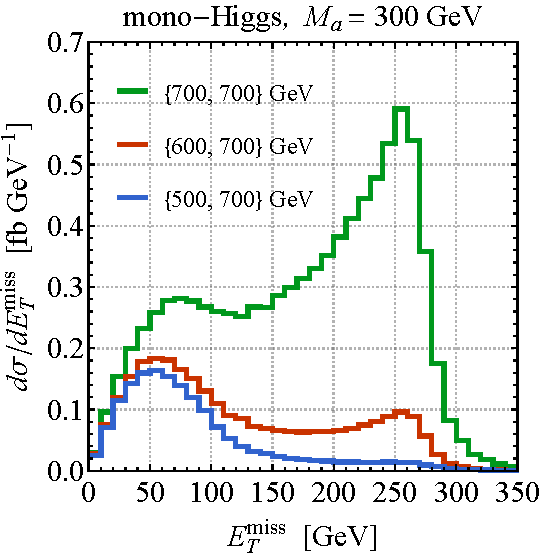
\includegraphics[height=0.45\textwidth]{texinputs/04_grid/newfigures/mvarl.pdf} \qquad 
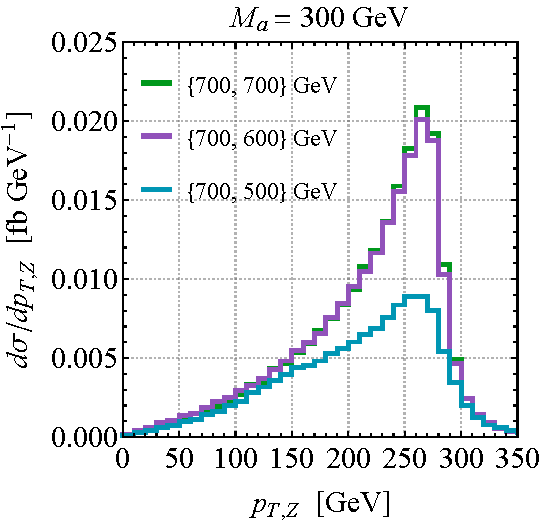
\includegraphics[height=0.45\textwidth]{texinputs/04_grid/newfigures/mvarr.pdf}
\vspace{2mm}
\caption{\label{fig:mvar} $\MET$ ($p_{T,Z}$) distributions for mono-Higgs~(mono-$Z$) production at $13 \, {\rm TeV}$ in the \hdma model.  The shown predictions  correspond to different sets $M_{H,A}$ of masses and employ $\mHc = {\rm min} \left ( \mH, \mA \right )$, $M_a = 300 \, {\rm GeV}$  as well as the parameters~\eqref{eq:benchmark}.}
\end{figure}

In Figure~\ref{fig:mvar} we display $\MET$ distributions in $h + \MET$ production~(left panel) and $p_{T,Z}$ distributions in $Z+\MET$ production~(right panel) for different~$\mH$ and~$\mA$ values. As~indicated, the coloured histograms correspond to  different choices of $M_{H,A}$ and $\mHc = {\rm min} \left ( \mH, \mA \right )$, but all employ $M_a = 300 \, {\rm GeV}$. From the figure it is evident that the inclusive mono-Higgs~(mono-$Z$) cross section is reduced compared to the benchmark prediction if~$\mH$~($\mA$) is taken to be smaller than $\mA$~($\mH$). 
%Numerically, we find  mono-Higgs and mono-$Z$ cross sections of $91 \, {\rm fb}$ ($16 \, {\rm fb}$) and $2.1 \, {\rm fb}$ ($1.3 \, {\rm fb}$) at $\sqrt{s} = 13 \, {\rm TeV}$, respectively. 
We furthermore observe that  a change of $\mH$ strongly affects the shape of the $\MET$ distribution, while the distortions in the $p_{T,Z}$ distribution under variations of~$\mA$ are much less pronounced. The strong $M_H$-dependence of the~$\MET$ spectrum in $h + \MET$ production can be traced back to the structure of the coupling~$g_{Aha}$. From~(\ref{eq:cubic}) one sees that for smaller~$M_H$ also $g_{Aha}$ is smaller, leading to a reduced $A \to ha$ branching ratio  and in turn to a lower rate of resonant production. In contrast, the coupling~$g_{HZa}$ that drives resonant production in the case of the mono-$Z$ signal does not depend on the value of~$M_A$. 

In order for resonant production to be dominant in both the $h + \MET$ and $Z + \MET$ case, we have chosen $\mH = \mA$ in the benchmark scenario~\eqref{eq:benchmark}. The further choice of having a common 2HDM Higgs mass $\mH = \mA = \mHc$ is then motivated by the observation that such an option minimises the constraints from EW precision observables and vacuum stability. See the discussion in Section~\ref{sec:constraints}. While in our sensitivity studies presented in the next section we will always employ the choice $\mH = \mA = \mHc$, in future \hdma  interpretations of mono-$X$ searches one might however  also want to consider cases with $\mH \neq \mA$. 

\subsection*{Variation of $\bm{\sin \theta}$}

\begin{figure}[t!]
\centering
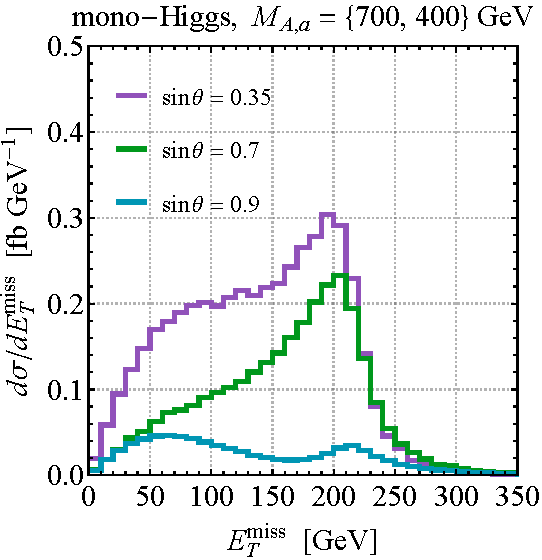
\includegraphics[height=0.45\textwidth]{texinputs/04_grid/newfigures/svarl.pdf} \qquad 
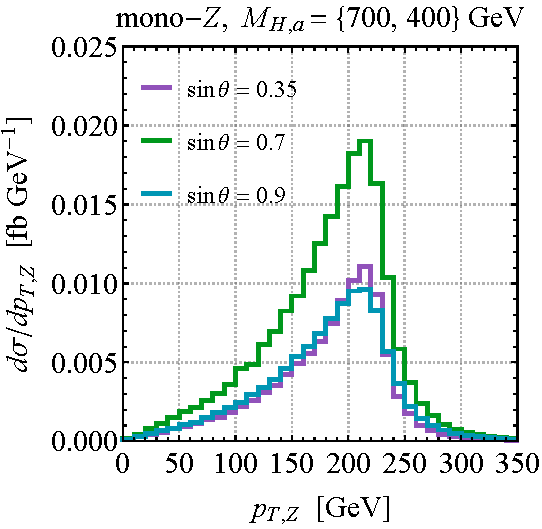
\includegraphics[height=0.45\textwidth]{texinputs/04_grid/newfigures/svarr.pdf}
\vspace{2mm}
\caption{\label{fig:svar} $\MET$ ($p_{T,Z}$) distributions for mono-Higgs~(mono-$Z$) production at $13 \, {\rm TeV}$  in the \hdma model. The displayed results correspond to different choices of $\sin \theta$. The remaining parameters are fixed to~\eqref{eq:benchmark} using $\mH = \mA = \mHc = 700 \, {\rm GeV}$ and $\ma = 400 \, {\rm GeV}$. }
\end{figure}

Figure~\ref{fig:svar} shows $\MET$ distributions in $h + \MET$ production~(left panel) and $p_{T,Z}$ distributions in $Z+\MET$ production~(right panel) for different~values of $\sin \theta$. The spin-0 masses are chosen as $\mH = \mA = \mHc = 700 \, {\rm GeV}$ and $\ma = 400 \, {\rm GeV}$, and the remaining parameters are fixed to~\eqref{eq:benchmark}. From the two panels it is evident that a variation of $\sin \theta$ leads to both a rate and shape change in the case of the mono-Higgs signal, while in the case of the mono-$Z$ channel only the total cross section gets rescaled to first approximation. The strong sensitivity of the shape of the $\MET$ spectrum in $h + \MET$ production is a again a result of the interplay of resonant and non-resonant contributions. While the $gg \to A \to h a \to h \chi \bar \chi$  amplitude scales as $\sin \theta \cos^3 \theta$, the $gg \to h a  \to h \chi \bar \chi$ matrix element shows a $\sin \theta \cos \theta$ dependence. These scalings imply that at small (large) $\sin \theta$ the resonant~(non-resonant) amplitudes provide the dominant contribution to the $\MET$ distribution in mono-Higgs production. In the case of the mono-$Z$ signal the resonant and non-resonant amplitudes both scale as $\sin \theta \cos \theta$ and in consequence the cross section and all kinematic distributions are essentially not distorted  under changes of the mixing angle~$\theta$. Notice that the latter statement also holds in the case of the $t \bar t +\MET$, $b \bar b + \MET$ and mono-jet signatures.  This can be deduced from~\eqref{eq:rescaling}. 

From the above discussion it follows that the choice $\sin \theta = 0.35$ made in~\eqref{eq:benchmark} leads to an enhanced sensitivity of the mono-Higgs signal to the \hdma parameter space. To perform parameter scans in scenarios with larger mixing angles like $\sin \theta = 0.7$ would however also be worthwhile because such a choice would lead to an improved coverage via the mono-$Z$ channel. We finally note that in scenarios with $\sin \theta >0.35$ the maximal allowed size of mass splitting $M_H - M_a$ is more constrained by vacuum stability arguments than in~\eqref{eq:benchmark}. This is can be seen from~\eqref{eq:BFB2}. 

\subsection*{Variation of $\bm{\tan \beta}$}

\begin{figure}[t!]
\centering
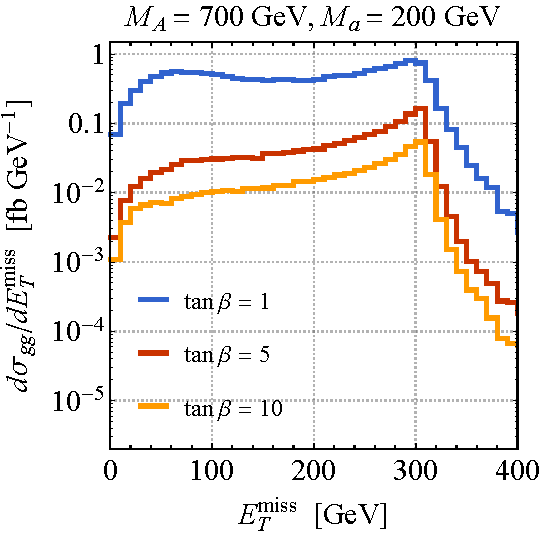
\includegraphics[height=0.45\textwidth]{texinputs/04_grid/newfigures/tbl.pdf} \qquad 
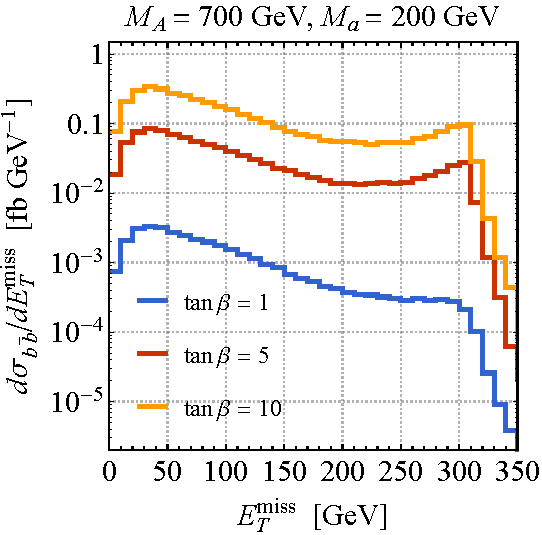
\includegraphics[height=0.45\textwidth]{texinputs/04_grid/newfigures/tbr.pdf}
\vspace{2mm}
\caption{\label{fig:tbvar} 
$\MET$ distributions for mono-Higgs production in $gg$-fusion (left panel) and $b \bar b$-fusion (right panel) in the \hdma model. The displayed results correspond to $pp$ collisions at  $13 \, {\rm TeV}$ and different choices of $\tan \beta$. The parameters not detailed in the plots are set to~\eqref{eq:benchmark} using $\mH = \mA = \mHc = 700 \, {\rm GeV}$ and $\ma = 200 \, {\rm GeV}$.}
\end{figure}

In Figure~\ref{fig:tbvar} we display $\MET$ distributions in mono-Higgs production for different choices of $\tan \beta$. The left (right) panel illustrates the contributions from the $gg \to h + \MET$ ($b \bar b \to h + \MET$) channel. The shown results have been obtained at $13 \, {\rm TeV}$ and employ~\eqref{eq:benchmark} with $\mH = \mA = \mHc = 700 \, {\rm GeV}$ and $\ma = 200 \, {\rm GeV}$. One first notices that the total production cross section in $gg$-fusion strongly decreases with increasing $\tan \beta$, while in the case of $b \bar b$-fusion the opposite behaviour is observed. The strong depletion/enhancement of the production rates originates from the fact that in  the type-II~\hdma model considered in this whitepaper the couplings of $H,A,a$ to top quarks are proportional to $\cot \beta$, while the corresponding couplings to bottom quarks are proportional to $\tan \beta$. Numerically, we find that for $\tan \beta \gtrsim 5$ the $gg$-fusion and $b\bar b$-fusion contributions to mono-Higgs production are comparable in size and thus both channels have to included to obtain accurate predictions. From the two panels it is furthermore apparent that variations of $\tan \beta$ do not only change the overall signal strength, but also have a pronounced impact on the shapes of the $\MET$ distributions. In particular, changes in $\tan \beta$ influence the importance of resonant versus non-resonant contributions. Like in the case of the mono-Higgs channel also for the mono-$Z$ signal $b \bar b$-initiated production can be relevant for sufficiently large values of $\tan \beta$~\cite{Bauer:2017ota}. {\color{red} [Uli: Show a plot here!]} The modifications in the kinematic distributions of $t \bar t + \MET$ and $j +\MET$ production under changes of $\tan \beta$ are compared to the mono-Higgs and mono-$Z$ signal less pronounced. 

Our  scans in the $M_{a}\hspace{0.5mm}$--$\hspace{0.5mm} M_H$ plane are based on the choice $\tan \beta = 1$, since for this value the existing mono-Higgs and mono-$Z$ searches already allow to probe/exclude large regions in the mass planes. In  future ATLAS and CMS analyses it would however be desirable that scans in $\tan \beta$ are carried out as well (cf. Section~\ref{sec:sensitivitystudies} and~\cite{No:2015xqa,Bauer:2017ota,Pani:2017qyd}). We add that in such a scan special attention has to be given to the fact that in the large-$\tan \beta$ limit the total decay widths of some of the Higgs states can become very large, potentially invalidating the NWA.

\subsection*{Variation of $\bm{m_\chi}$}

\begin{figure}[t!]
\centering
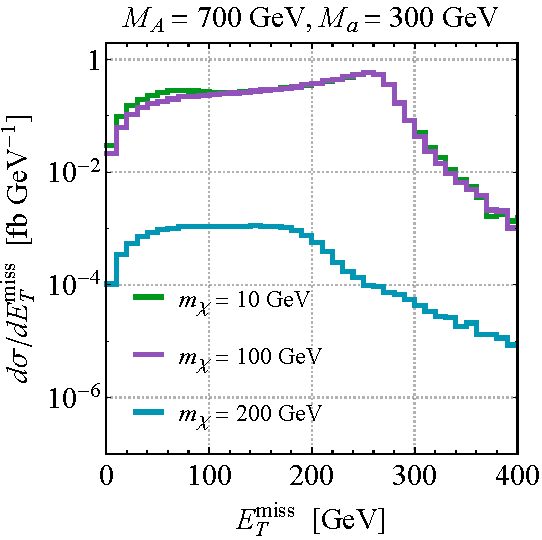
\includegraphics[height=0.45\textwidth]{texinputs/04_grid/newfigures/mdml.pdf} \qquad 
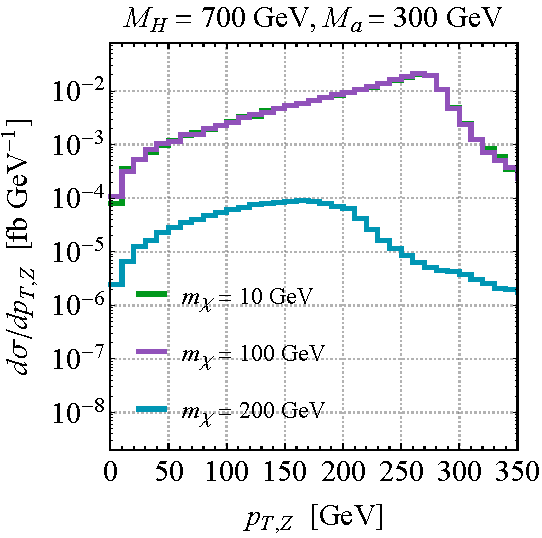
\includegraphics[height=0.45\textwidth]{texinputs/04_grid/newfigures/mdmr.pdf}
\vspace{2mm}
\caption{\label{fig:mdmvar} $\MET$ ($p_{T,Z}$) distributions for mono-Higgs~(mono-$Z$) production at $13 \, {\rm TeV}$. The presented results correspond to different values of the DM mass $m_\chi$. The other \hdma parameters are set to~\eqref{eq:benchmark} using $\mH = \mA = \mHc = 700 \, {\rm GeV}$ and $\ma = 300 \, {\rm GeV}$. }
\end{figure}

The modifications of the $\MET$~($p_{T,Z}$) spectrum in $h+\MET$~($Z+\MET$) production under a variation of the DM mass $m_\chi$ are illustrated in the two panels of Figure~\ref{fig:mdmvar}. The given predictions correspond to $pp$ collision at $13 \, {\rm TeV}$ and employ the benchmark parameters~\eqref{eq:benchmark} with $\mH = \mA = \mHc = 700 \, {\rm GeV}$ and $\ma = 300 \, {\rm GeV}$. One observes that the depicted scenarios with $\ma  > 2 m_\chi$ (green and purple histograms) lead to almost identical rates, $\MET$ and $p_{T,Z}$ spectra, while the choice $\ma  < 2 m_\chi$ (blue histograms) 
largely reduces the total rates and also modifies the shapes of the shown distributions. This feature is expected since for $\ma > m_\chi/2$ ($\ma < m_\chi/2$) the decay channel $a \to \chi \bar \chi$ is kinematically allowed~(forbidden). In order to have detectable mono-$X$ signals even for light mediators~$a$, we have chosen a value of  $m_\chi = 10 \, {\rm GeV}$ as the baseline for the following sensitivity studies. %{\color{red} [Uli: Comment on relic density here? Or only later?]}

\section{Non-$\bm{E_T^{\rm miss}}$ collider signatures}
\label{sec:nonMET}

In this section we will discuss the most important non-$\MET$ signals that can be used to explore the parameter space of the \hdma model at the LHC. Most of the discussion will be centred around final states containing top quarks since these channels provide the best sensitivity to model realisations with low $\tan \beta$ such as our benchmark parameter choice~\eqref{eq:benchmark}. Final states that give excess to the \hdma parameter space with large $\tan \beta$ such as di-tau searches will however also be discussed briefly. 

\subsection{Di-top  searches}
\label{sec:ttbarresonances}

In all 2HDM models, the spin-0 bosons $H,A$  decay dominantly to top-quark pairs if these states have masses above the top-quark threshold,~i.e.~$M_{H, A} > 2 m_t$, and if $\tan \beta = {\cal O}(1)$. New-physics scenarios of this kind can thus be tested by studying the $t \bar t$ invariant mass spectrum $m_{t \bar t}$.  Interference effects between the signal process and the SM  $t \bar t$ background however distort the $m_{t \bar t}$ signal shape from a single peak to a peak-dip structure~\cite{Gaemers:1984sj,Dicus:1994bm,Bernreuther:1997gs,Frederix:2007gi,Hespel:2016qaf}, a feature that represents a serious obstacle to probe 2HDM models with $M_{H,A} > 350 \, {\rm GeV}$ and small $\tan \beta$ values~\cite{Craig:2015jba,Hajer:2015gka,Gori:2016zto,Carena:2016npr}. 

\begin{figure}
\centering
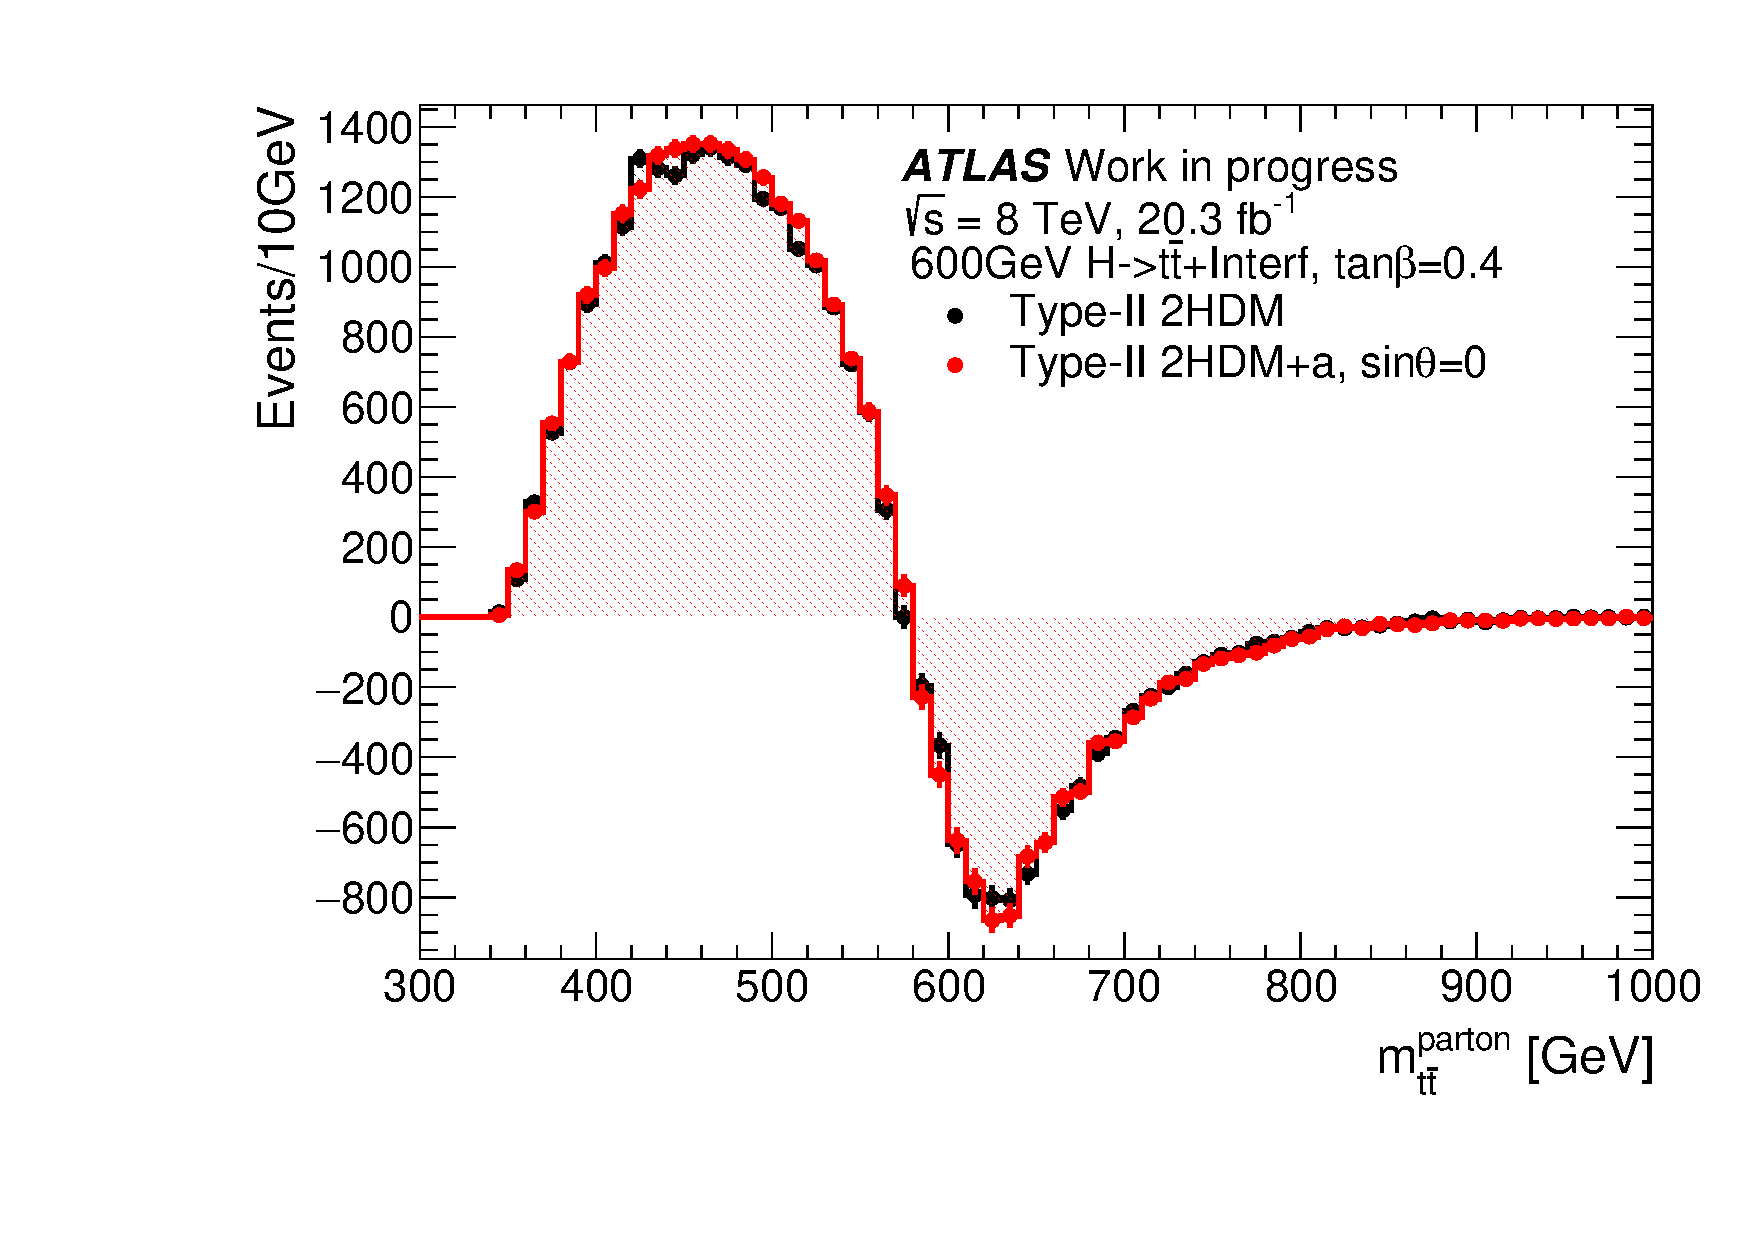
\includegraphics[width=.48\textwidth]{texinputs/04_grid/figures/ttres/ttres_2HDMvs2HDMa_H.pdf} \quad 
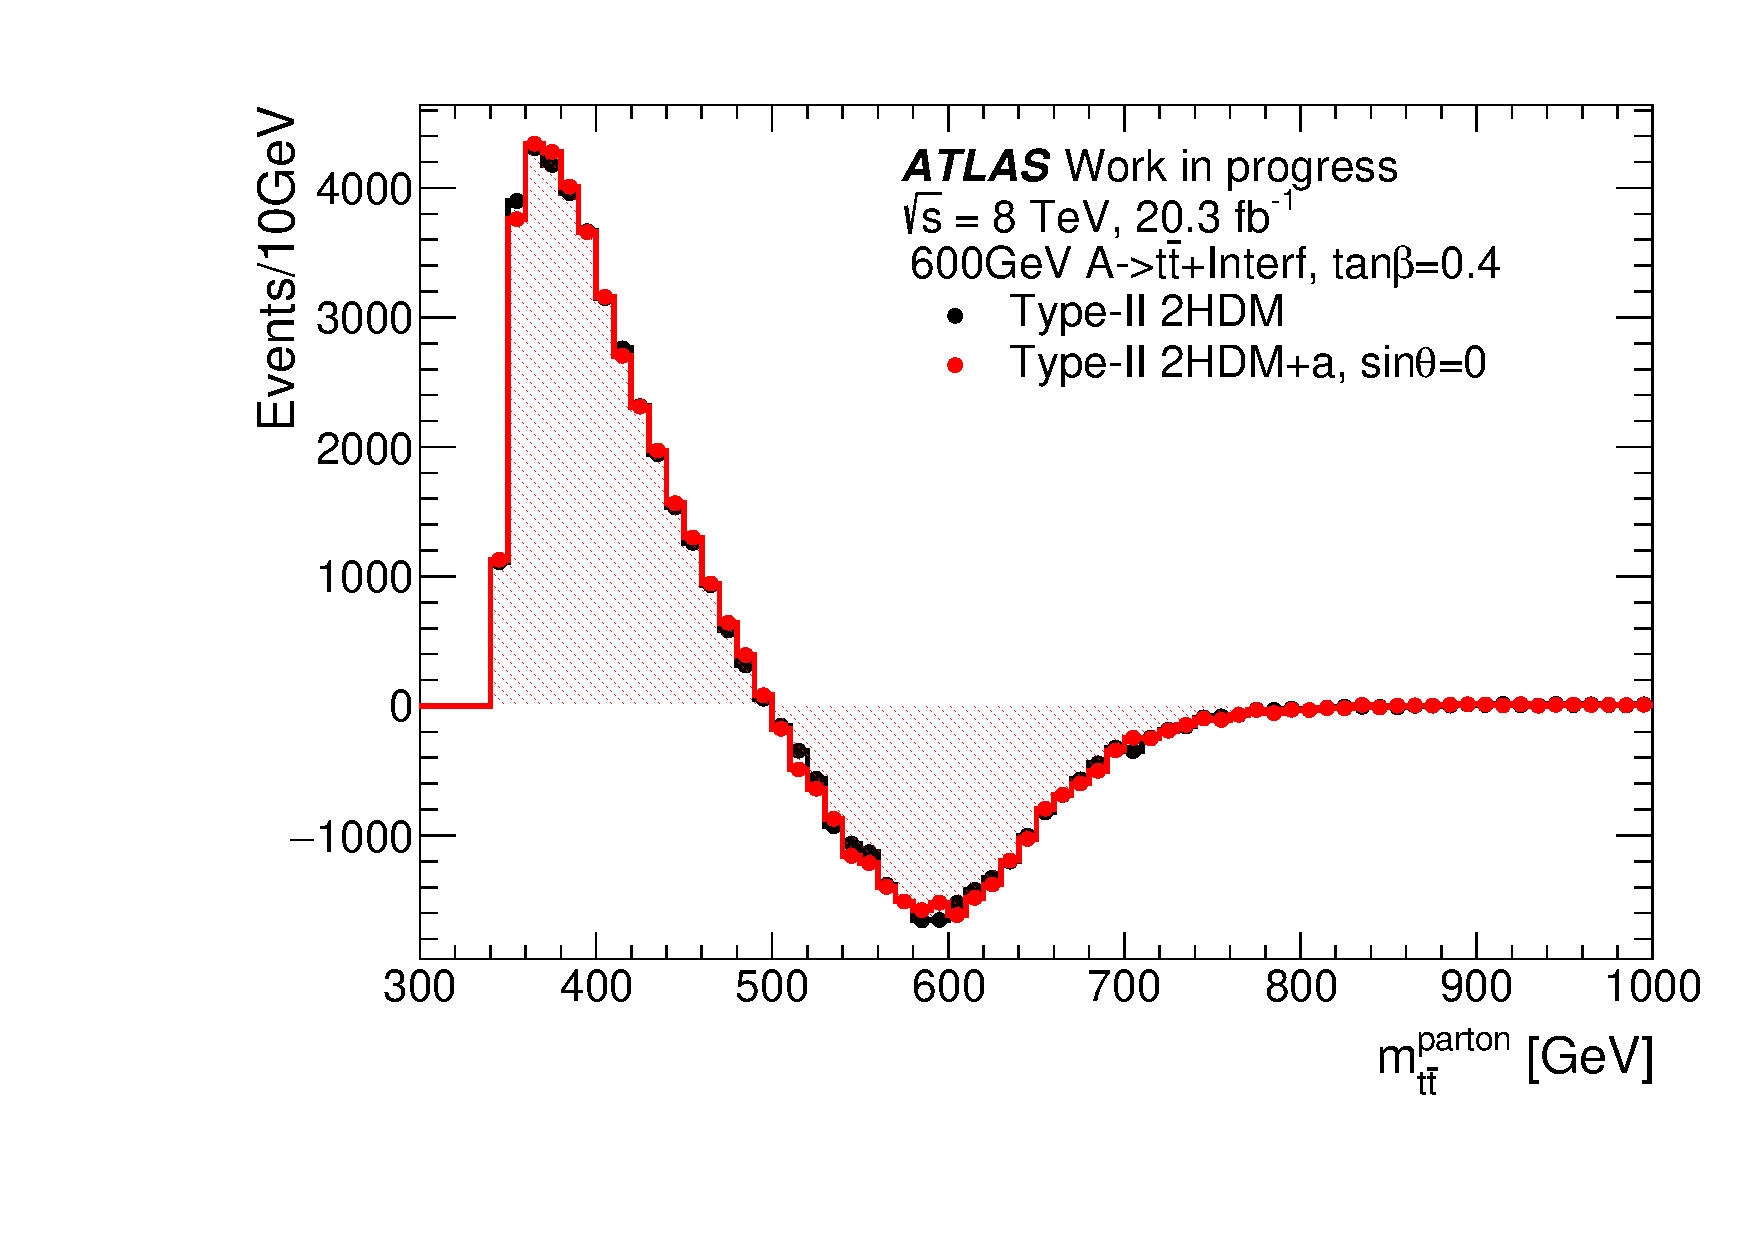
\includegraphics[width=.48\textwidth]{texinputs/04_grid/figures/ttres/ttres_2HDMvs2HDMa_A.pdf}
\caption{$m_{t \bar t}$ spectra for $gg \to H \to t \bar t$~(left) and  $gg \to A \to t \bar t$~(right). The black (red) predictions correspond to the type-II 2HDM (\hdma) model.  The shown results employ $\mA=\mH=600 \, {\rm GeV}$,  $\ma=100 \, {\rm GeV}$, $\tan \beta =0.4$ and $\sin \theta = 0$.  {\color{red} [Uli: Fix notation etc.!]}}
\label{fig:ttres_2HDMvs2HDMa}
\end{figure}

The ATLAS search in Ref.~\cite{Aaboud:2017hnm} takes into account interference effects between the signal process $gg \to H/A \to t \bar t$ and the SM background $gg \to t \bar t$ is the . This search is based on an integrated luminosity of $20.3 \, {\rm fb}^{-1}$ collected at $8 \, {\rm TeV}$ and interprets results in the alignment limit of a type-II 2HDM without a pseudoscalar decaying to DM. The obtained  exclusion limits in the $M_{H,A}\hspace{0.5mm}$--$\hspace{0.5mm} \tan \beta$ plane are stronger than previously published LHC constraints on the 2HDM parameter space with low $\tan \beta$ and $M_{H,A} \in [500, 650] \, {\rm GeV}$. For instance,  for $M_{H,A} = 500 \, {\rm GeV}$ values of $\tan \beta < 1$ are disfavoured at 95\%~CL. A~similar parameter space  can be probed if the results~\cite{Aaboud:2017hnm} are reinterpreted in the context of the \hdma model~\cite{Bauer:2017ota}. The di-top invariant mass spectra obtained in the \hdma model as a function of different model parameters is shown in Figures~\ref{fig:ttres_2HDMvs2HDMa} and \ref{fig:ttres_2HDM_A}. 


{\color{red} [Uli: Work in progress!]}

 A similar kinematic range could be probed if the result were re-interpreted in the context of the \hdma. Interference between
a loop-induced and a tree-level process cannot currently be simulated in \mg. To amend this problem, the same "Higgs\_Effective\_Couplings\_FormFactor"
approach \cite{ttinterfHFF} as adopted in \cite{Aaboud:2017hnm} is implemented in the UFO, replacing the loop production by an 
effective vertex. The predictions of the modified UFO for the case, in which the pseudoscalar mediator does not mix with the heavy pseudoscalar $A$ ($\sinp=0$), i.e. effectively decouples from the 2HDM Higgs sector, are compared to those for the minimal 2HDM. Excellent agreement is found in the invariant mass distributions of $A/H$ decaying into a top pair are shown in Fig.~\ref{fig:ttres_2HDMvs2HDMa}. As examples of how the sensitivity changes as a function of the parameters of the \hdma, the $M_{\ttbar}$ distributions of pseudoscalars decaying into \ttbar\ are presented in Fig~\ref{fig:ttres_2HDM_A}. Larger values of \tanb\ or \sinp\ are expected to yield lower sensitivities to $A\rightarrow\ttbar$ significantly while \ma\ almost only affects the contribution from $a\rightarrow\ttbar$, which becomes sizeable if \ma is close to $2\mt$.


\begin{figure}
\centering
\begin{subfigure}[b]{0.49\textwidth}
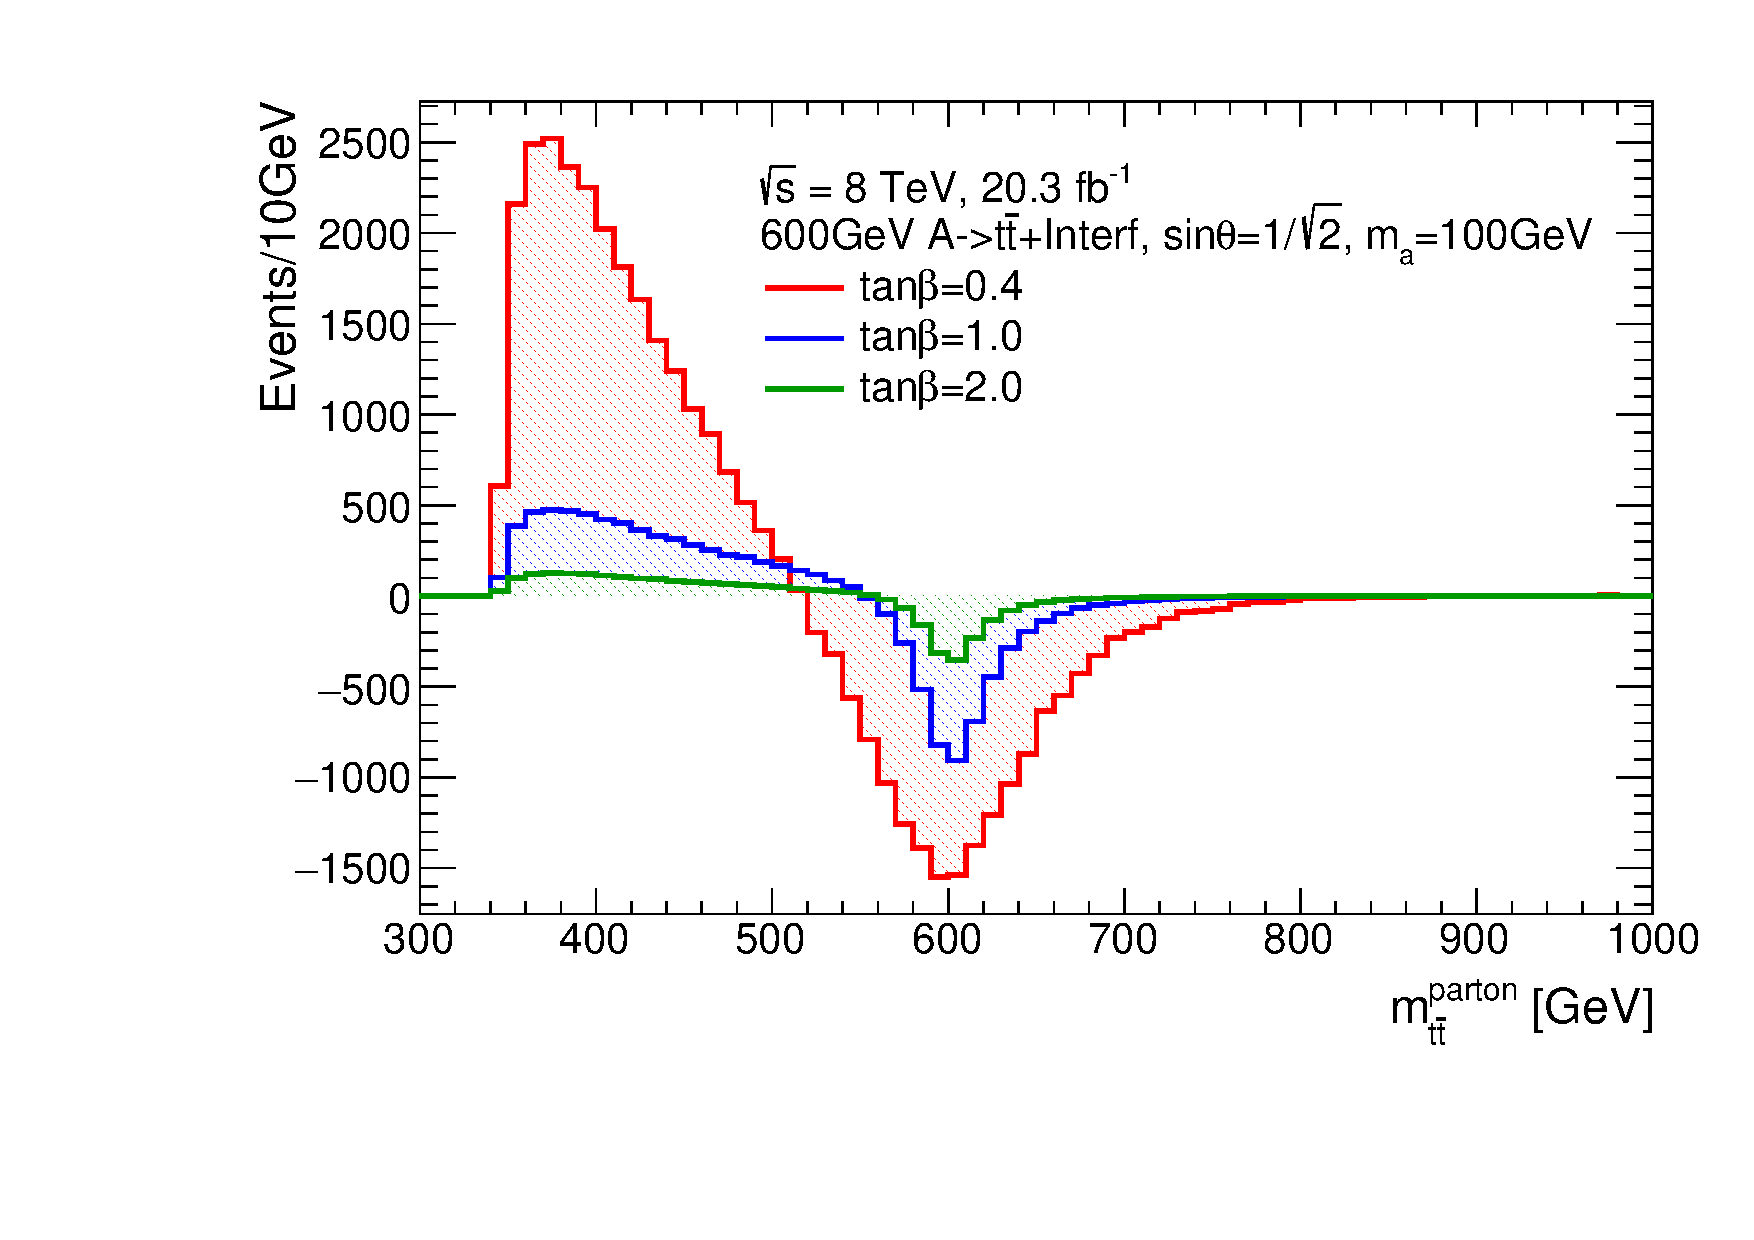
\includegraphics[width=\textwidth]{texinputs/04_grid/figures/ttres/ttres_2HDMa_A_tanb.pdf}
\caption{\tanb dependency with fixed $\sinp=1/\sqrt{2}$ and $\ma=100\GeV$}
\end{subfigure}
\begin{subfigure}[b]{0.49\textwidth}
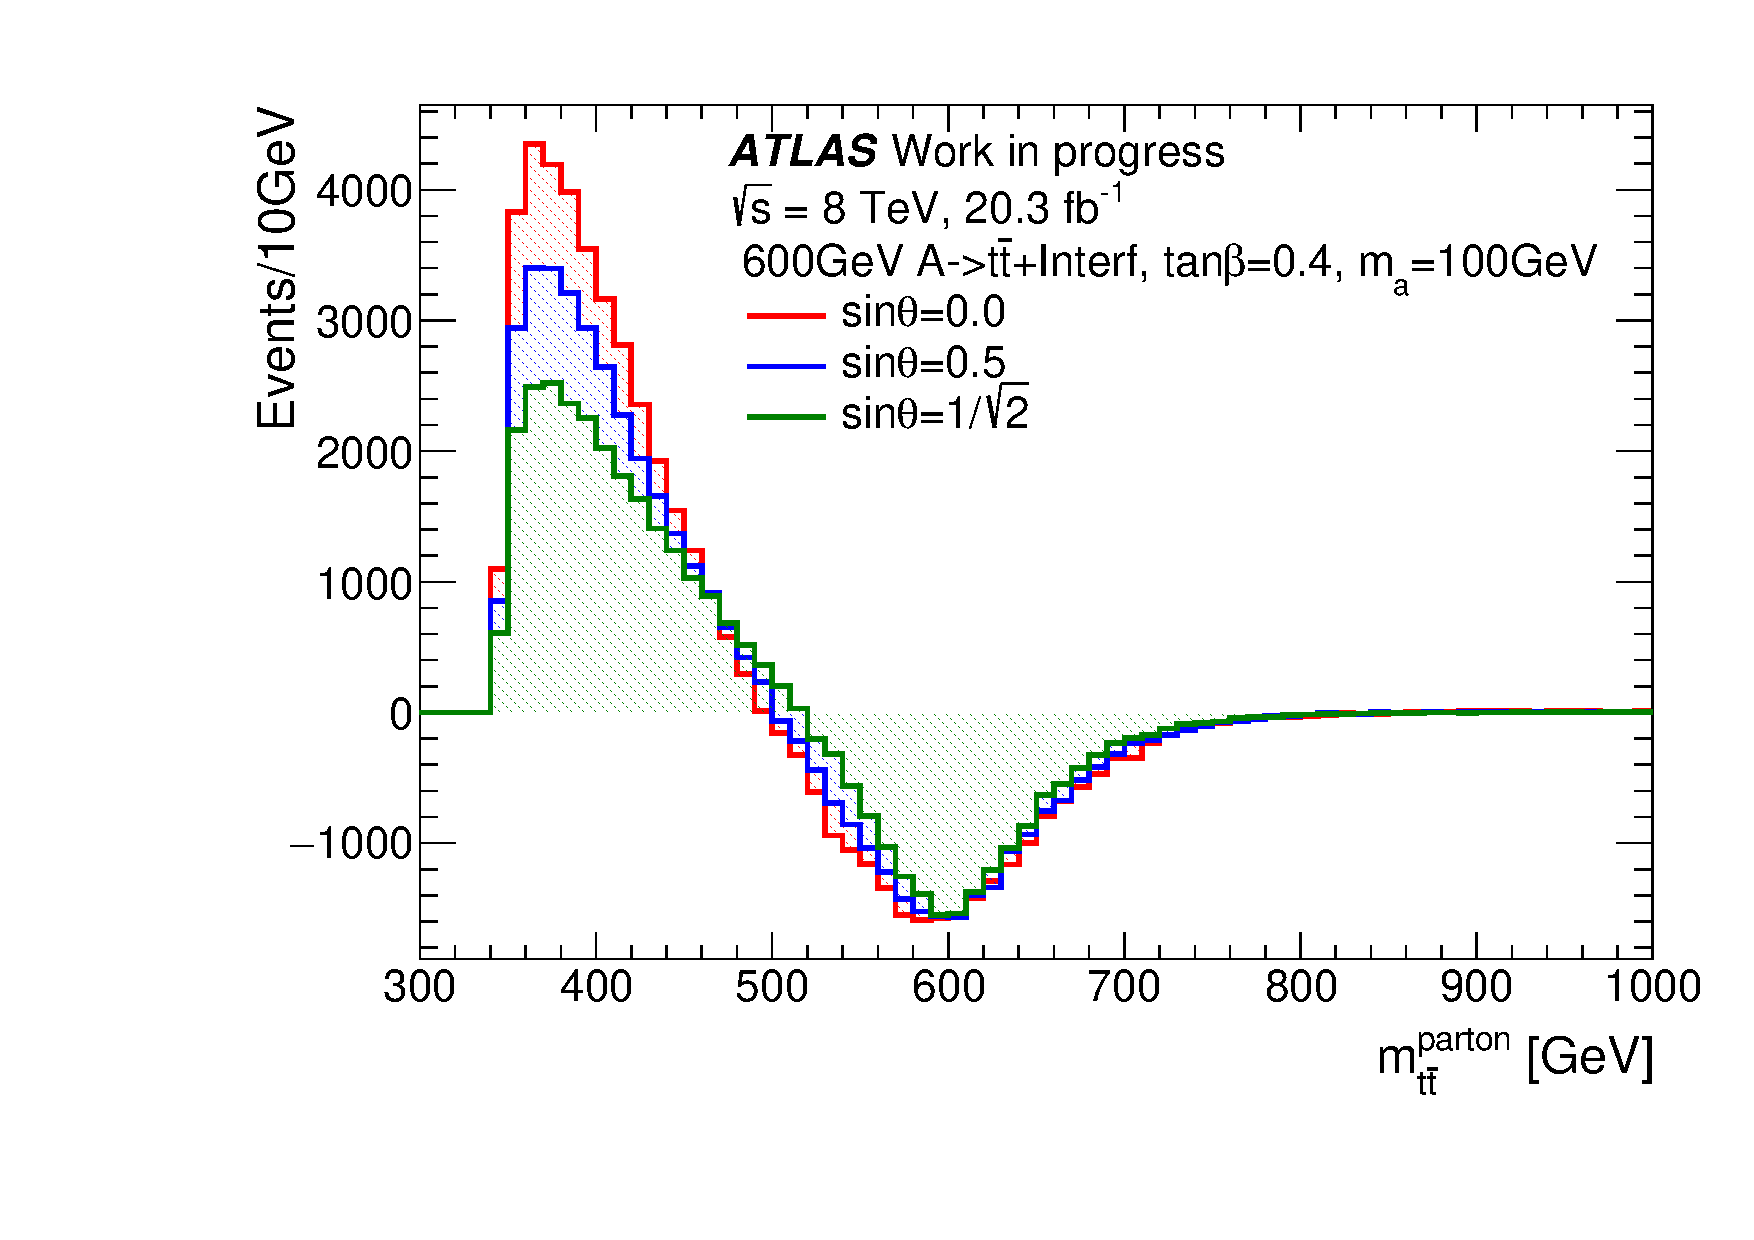
\includegraphics[width=\textwidth]{texinputs/04_grid/figures/ttres/ttres_2HDMa_A_sinp.pdf}
\caption{\sinp dependency with fixed $\tanb=0.4$ and $\ma=100\GeV$}
\end{subfigure}
\begin{subfigure}[b]{0.49\textwidth}
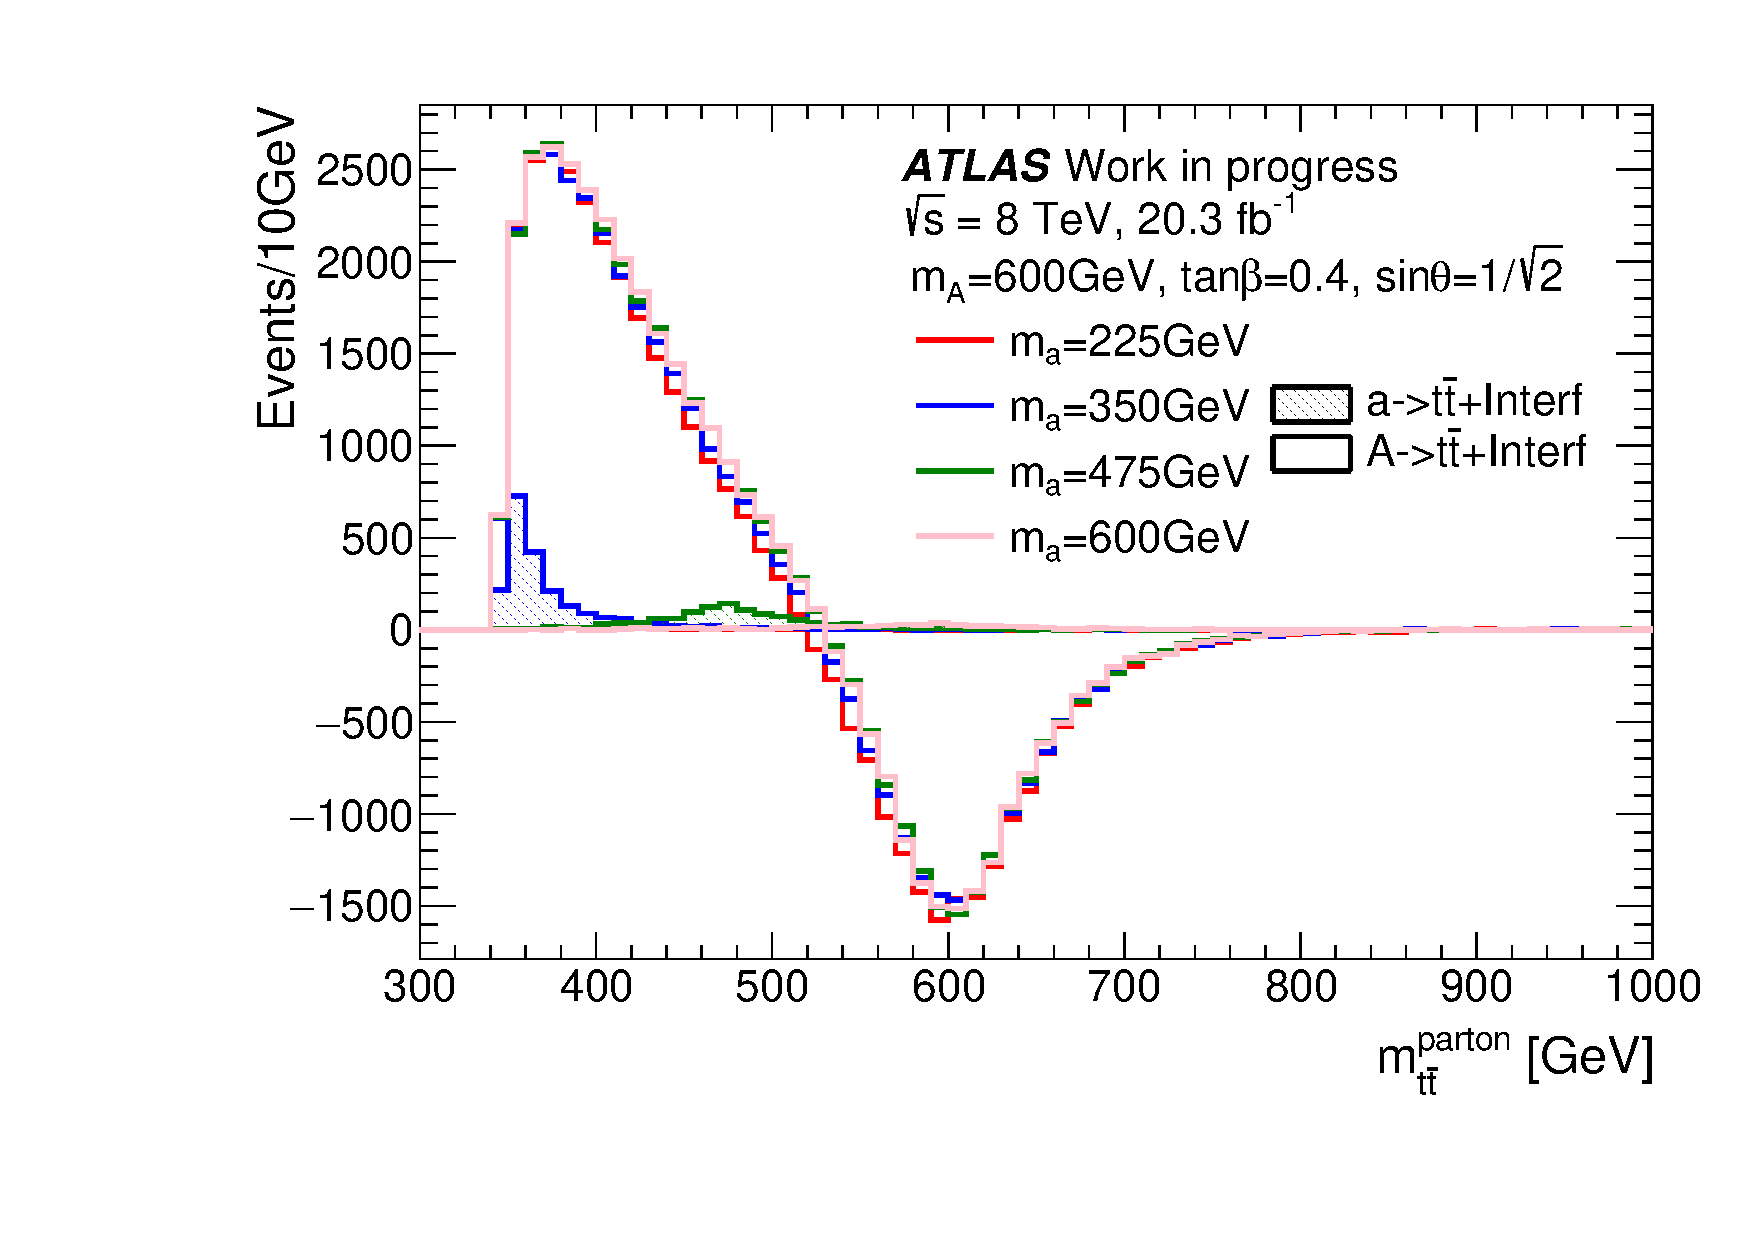
\includegraphics[width=\textwidth]{texinputs/04_grid/figures/ttres/ttres_2HDMa_A_ma.pdf}
\caption{\ma dependency with fixed $\tanb=0.4$ and $\sinp=1/\sqrt{2}$}
\end{subfigure}
\caption{parameter dependency of signal $M_{\ttbar}$ distribution mediated by pseudosalars. The value of \mA is fixed at 600\GeV.}
\label{fig:ttres_2HDM_A}
\end{figure}


\subsection{Four-top searches}

The topology involving four top-quarks in the final state is a rare,
yet increasingly important signature, which will gain sensitivity and
attention with the enlargement of the dataset delivered by the LHC.  
In the attempt to perform a first characterisation of this topology,
we have studied the predicted cross-section for the four top final
state of this model for two sets of parameter choices. 

In Figure~\ref{DMHF-4top-scan1} we present the four top cross section
for the parameter choices for the parameter choices
of \sinp = 0.35, \mA = \mH = \mHc = 600 GeV, for an intermediate choice
of mass of the light pseudoscalar ($m(a) = 400$ GeV), as a function of
$tan\beta$. 
\color{red}[Caterina: this may be too technical?]\color{black}
The total four-top production cross section, which
accounts for both SM and new physics (NP) contributions and is indicated
as $|SM+NP|^2$ in the legend, is compared with the production cross
section contributions separately due to SM and NP terms. 
This is achieved technically by setting a requirement on the number of
QCD and QED vertices in madgraph, as indicated in Table~\ref{tab-dmhf-4tops}.
%CD: removed, not clear to me where things are indicated
%Furthermore, the different contributions from on-shell production of
%each CP-odd and CP-even mediators associated with a top pair and
%decaying into a top pair is indicated. 
The dominant contribution is
driven by the on-shell production of $A$ and $H$ for all choices of
$tan\beta$ in this benchmark. 
In the lower panel of Figure~\ref{DMHF-4top-scan1}, the effect of the
interference term between the 2HDM+a and the SM is assessed, and is
found to have an impact almost always smaller than 5\% on the
inclusive cross-section. 
We note however that the validity of this statement depends
on the selection in the experimental analysis. 

\color{red}[Caterina: clarify what benchmark 3a and 3b are in the following?]\color{black}
In Figure~\ref{DMHF-4top-scan2} we present the cross-section
study when using $sin\theta = \frac{1}{\sqrt{2}}$, as a function of the light
pseudoscalar mass. 
For these parameter choices the cross-section is
independent of $m(a)$. As it can
be observed from the on-shell contribution breakdown, at the
low-end of the mass spectrum the $\ttbar+a$ production dominates, with a
peak at $400$ GeV due to the competition between
$a\rightarrow \chi\chi$ and $a\rightarrow \ttbar$ and the 
decreasing of the cross section with the increase of $m(a)$.  The contribution of
$\ttbar+H$ and $\ttbar+A$ processes compensates the latter effect in
the higher end of the mass-spectrum, with the turn on starting around
$800$ GeV due to the competition between $A/H\rightarrow\ttbar$ and
cascade decays of the heavy higgses into the light pseudoscalar
mediator ($A\rightarrow ah/H\rightarrow aZ$). 
The small feature at 1 TeV is due to interference effects between the
three higgs mediators, which are all set to the
same mass for this parameter choice.  
The inclusive production cross-section of the \hdma
model is also compared with the one obtained by the \texttt{DMSimp} pseudoscalar
implementation. 
Similarly to the previous benchmark points, the impact of the SM interference term on the inclusive cross-section is found to be very small ($<2\%$), except for $m(a)$ values close to the top theshold. 

Finally, in Figure~\ref{DMHF-4top-scan3} we compare for a small $\tan\beta$ value, the cross section of four-top production from NP processes (see Tab.~\ref{tab-dmhf-4tops}) of benchmarks \#3a and \#3b. This cross-section increases for benchmark \#3b for increasing $sin\theta$, as the production mechanism is dominated by $\ttbar+a(\ttbar)$. A different and more flat trend is instead observed for benchmark \#3a, for which the $sin\theta$ dependence is more complex and driven by the branching ratios of $A$ and $H$ in a top pair, as the $a\rightarrow \ttbar$ threshold is closed in this case. 

\begin{table}
\begin{tabular}{ccm{50mm}}
\toprule
{\sc Madgraph} rule & Legend symbol & Details \\\midrule
\verb| p p > t t~ t t~ / a z h1 QED<=2|& $|SM+NP|^2$ & Four-top
production including both SM and NP contributions and their
interference. \\\midrule
\verb| p p > t t~ t t~ / a z h1 QCD<=2|& $|NP|^2$ & Four-top
production from NP processes, including interference terms among
$A,H,a$. \\\midrule
\verb| p p > t t~ t t~ / a z h1 QED<=0|& $|SM|^2$ & Four-top SM
production.\\
\bottomrule
\end{tabular}
\caption{Description of the specific MADGRAPH settings used to derive
the different curves of Figs~\ref{DMHF-4top-scan1}~and~\ref{DMHF-4top-scan2}.}
\label{tab-dmhf-4tops}
\end{table}

\begin{figure}
\centering
\begin{subfigure}[b]{0.8\textwidth}
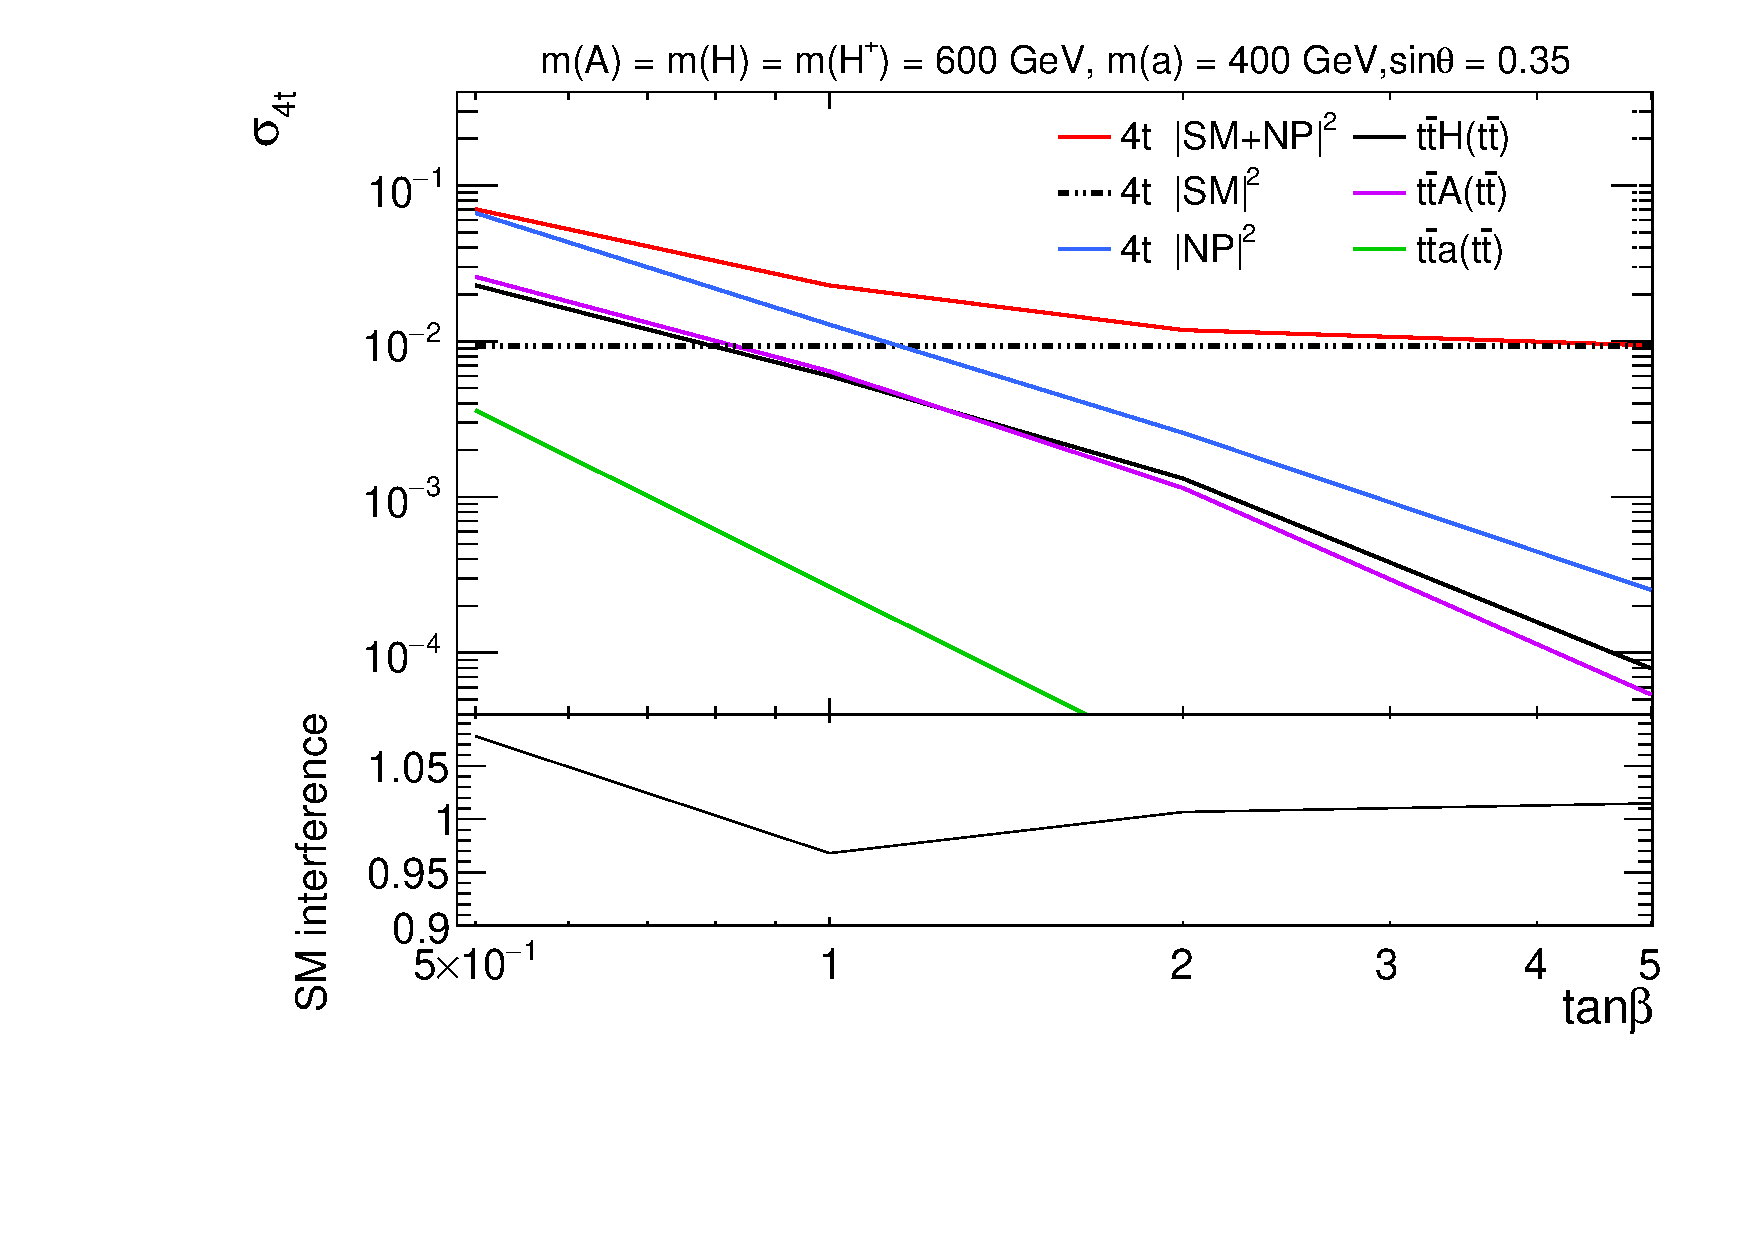
\includegraphics[width=\textwidth]{texinputs/04_grid/figures/DMHF/4tops/WHP_final_tbscan.pdf}
\caption{}
\label{DMHF-4top-scan1}
\end{subfigure}
\begin{subfigure}[b]{0.8\textwidth}
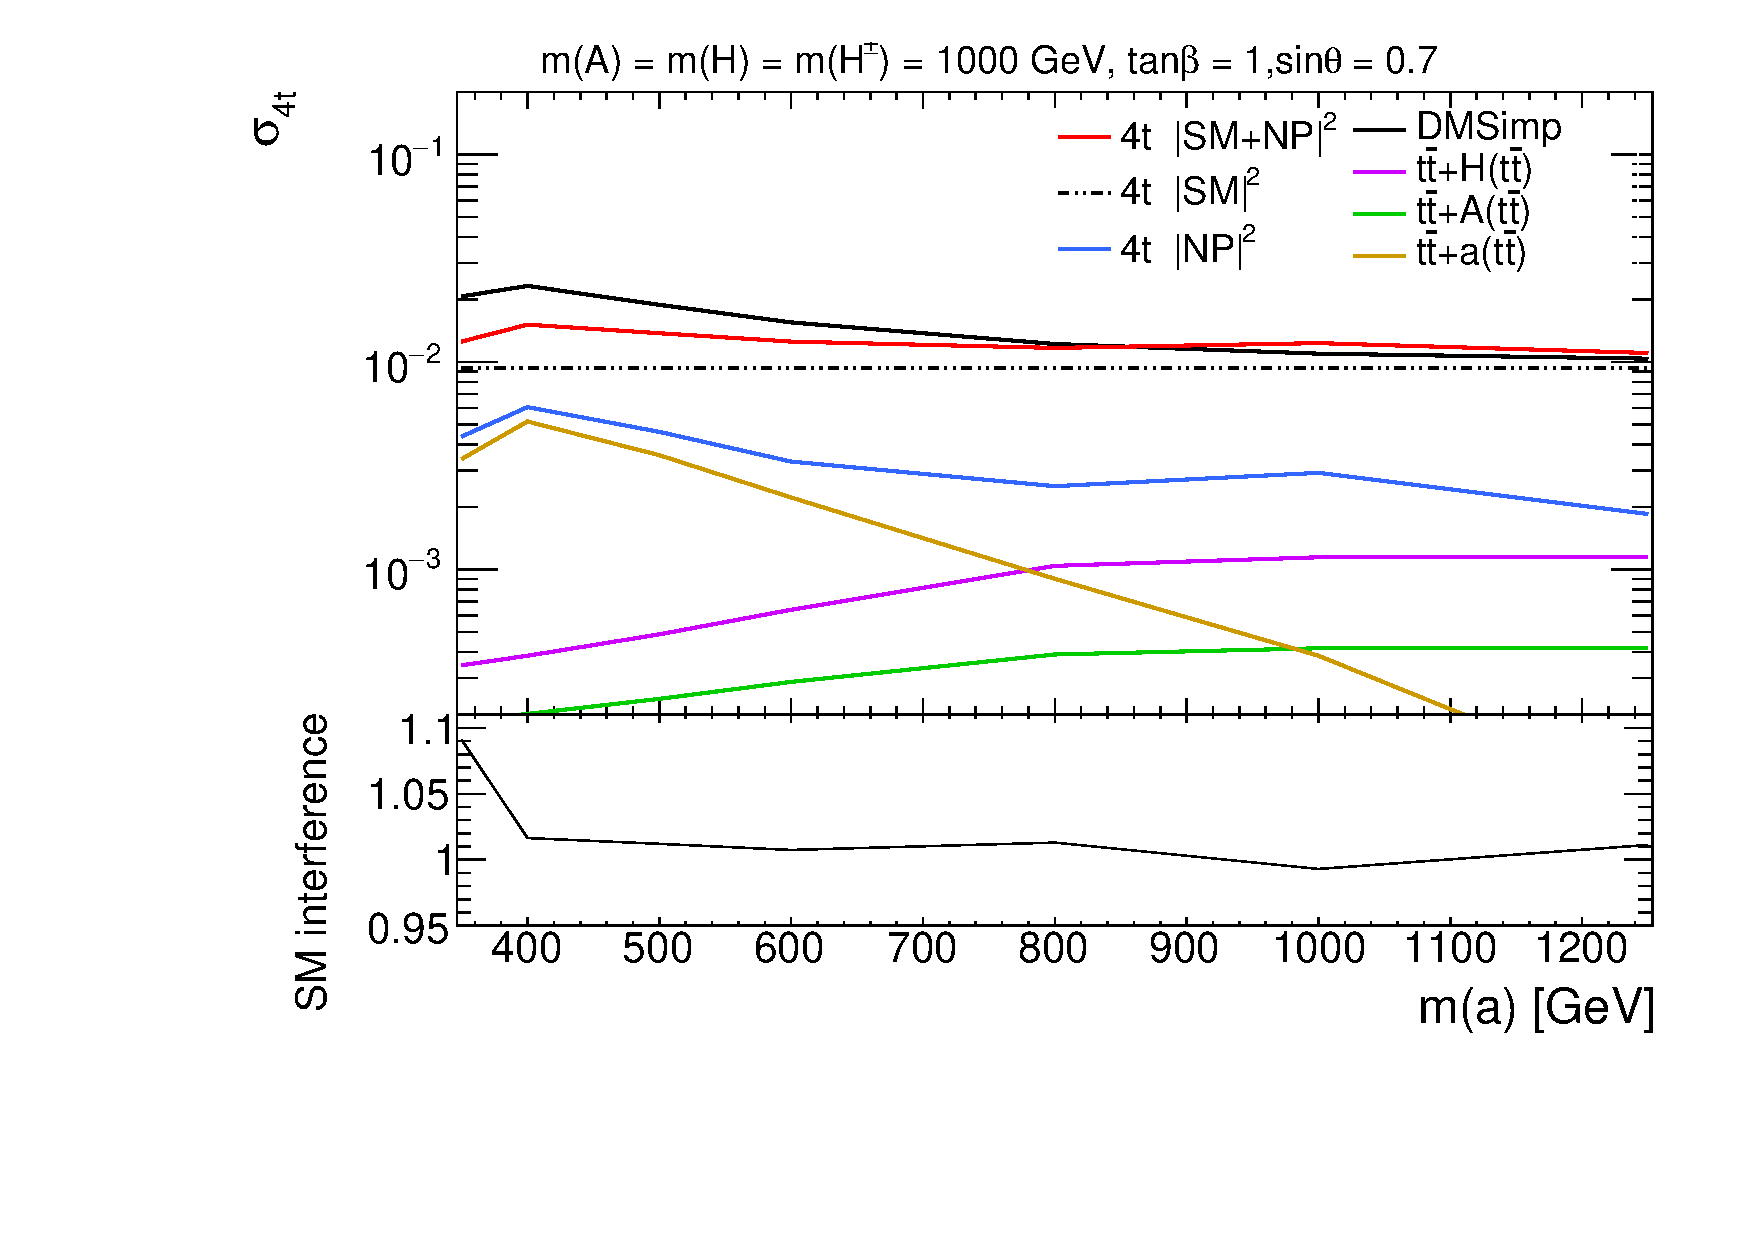
\includegraphics[width=\textwidth]{texinputs/04_grid/figures/DMHF/4tops/WHP_final_mascan.pdf}
\caption{}
\label{DMHF-4top-scan2}
\end{subfigure}
\caption{Four-top cross section study for a subset of the parameter
space of benchmark \#2 (top) and \#3 (bottom). The different Standard
Model (SM) and New Physics (NP) contributions with and without
interference and the breakdown in terms of on-shell mediator
production is presented, following the notation of Table~\ref{tab-dmhf-4tops}. }
\end{figure}

\begin{figure}
\centering
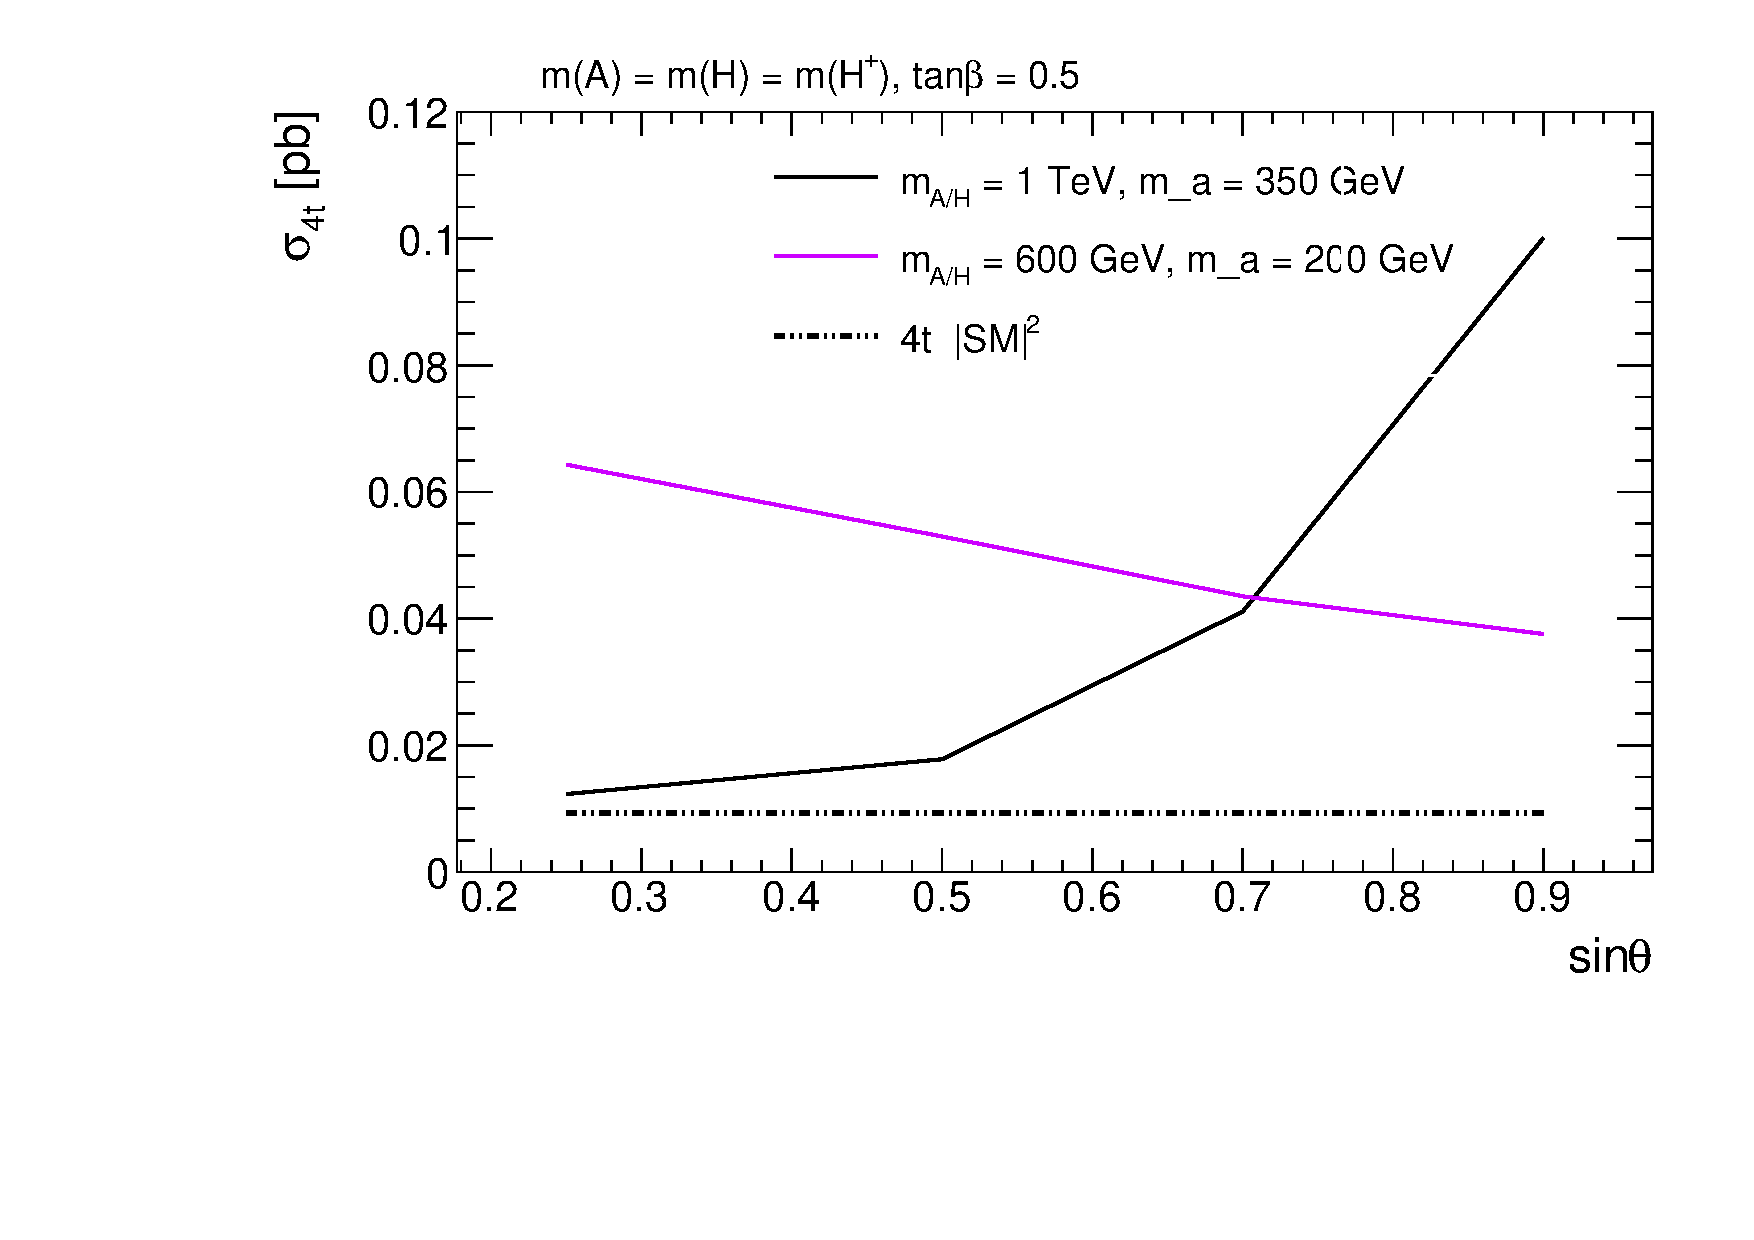
\includegraphics[width=.8\textwidth]{texinputs/04_grid/figures/DMHF/4tops/WHP_final_stscan.pdf}
\caption{Four-top cross section comparison for benchmarks \#3a and \#3b. Only NP contribution is presented, following the notation of Table~\ref{tab-dmhf-4tops}.}
\label{DMHF-4top-scan3}
\end{figure}

\subsection{Other final states}
\label{sec:others}

\section{Sensitivity studies}
\label{sec:sensitivitystudies}

In this section we present sensitivity estimates for two of the main $\MET$ signatures in the \hdma model, namely the $h +\MET$  and the $Z+\MET$ channels. Specifically, we will consider the mono-Higgs (mono-$Z$) signal in the $b \bar b$ ($\ell^+ \ell^-$) channel. Our studies are based on generator-level reinterpretation of existing results with  $36 \, {\rm fb}^{-1}$ of LHC data taken at $\sqrt{s} = 13 \, {\rm TeV}$. These results contain different amounts of public information. In the mono-Higgs case model-independent limits presented in~\cite{Aaboud:2017yqz} are used for the reinterpretation, while in the mono-$Z$ case  the sensitivity is estimated using generator-level information on the signal together with published background estimates~\cite{Aaboud:2017bja}. The sensitivities that other~$\MET$ searches provide are also briefly discussed below.  

\subsection{Mono-Higgs study}
\label{sec:sensi_monohbb}

\begin{figure}[t!]
\centering
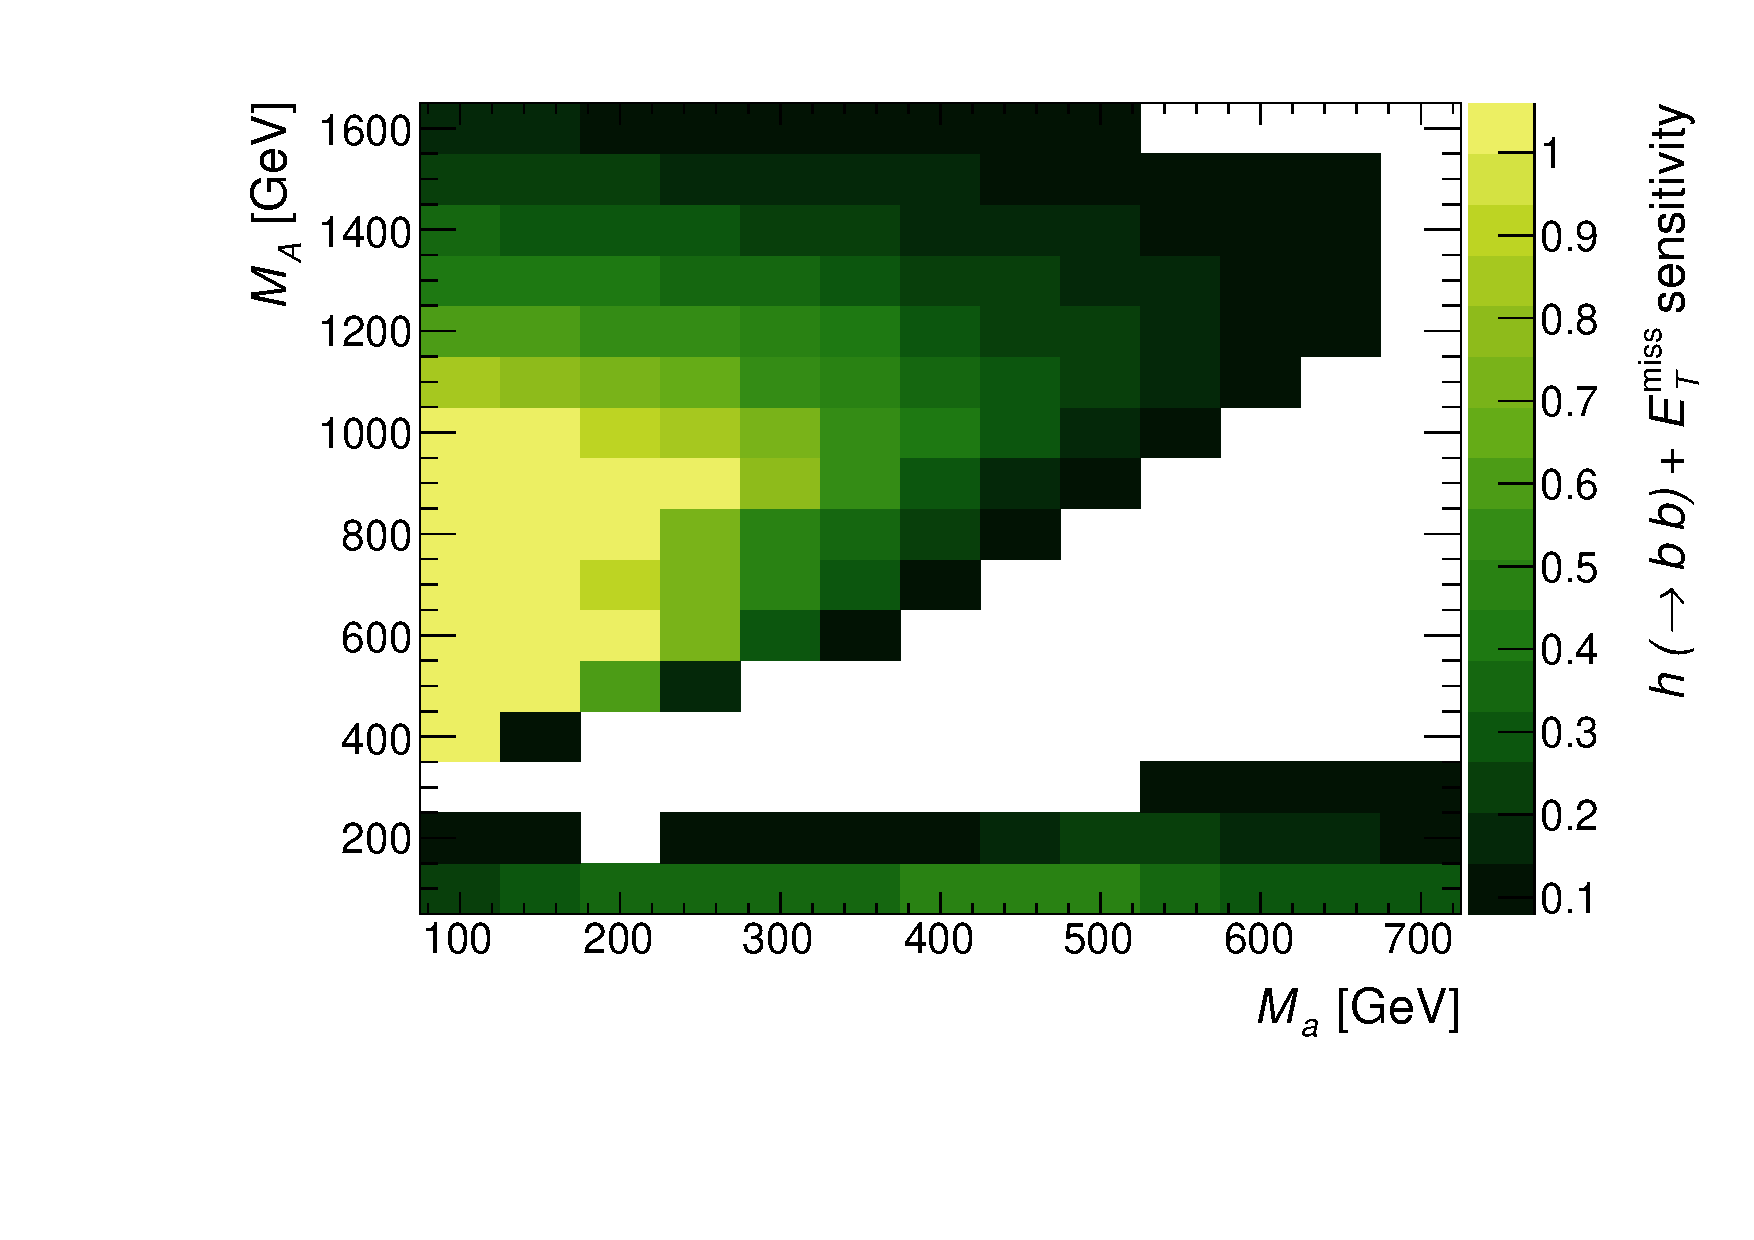
\includegraphics[width=0.75\textwidth]{texinputs/04_grid/figures/monoHbb_sensi_sum_bins_1_2_3_4_ma_vs_mA_lin.pdf}

\vspace{2mm}

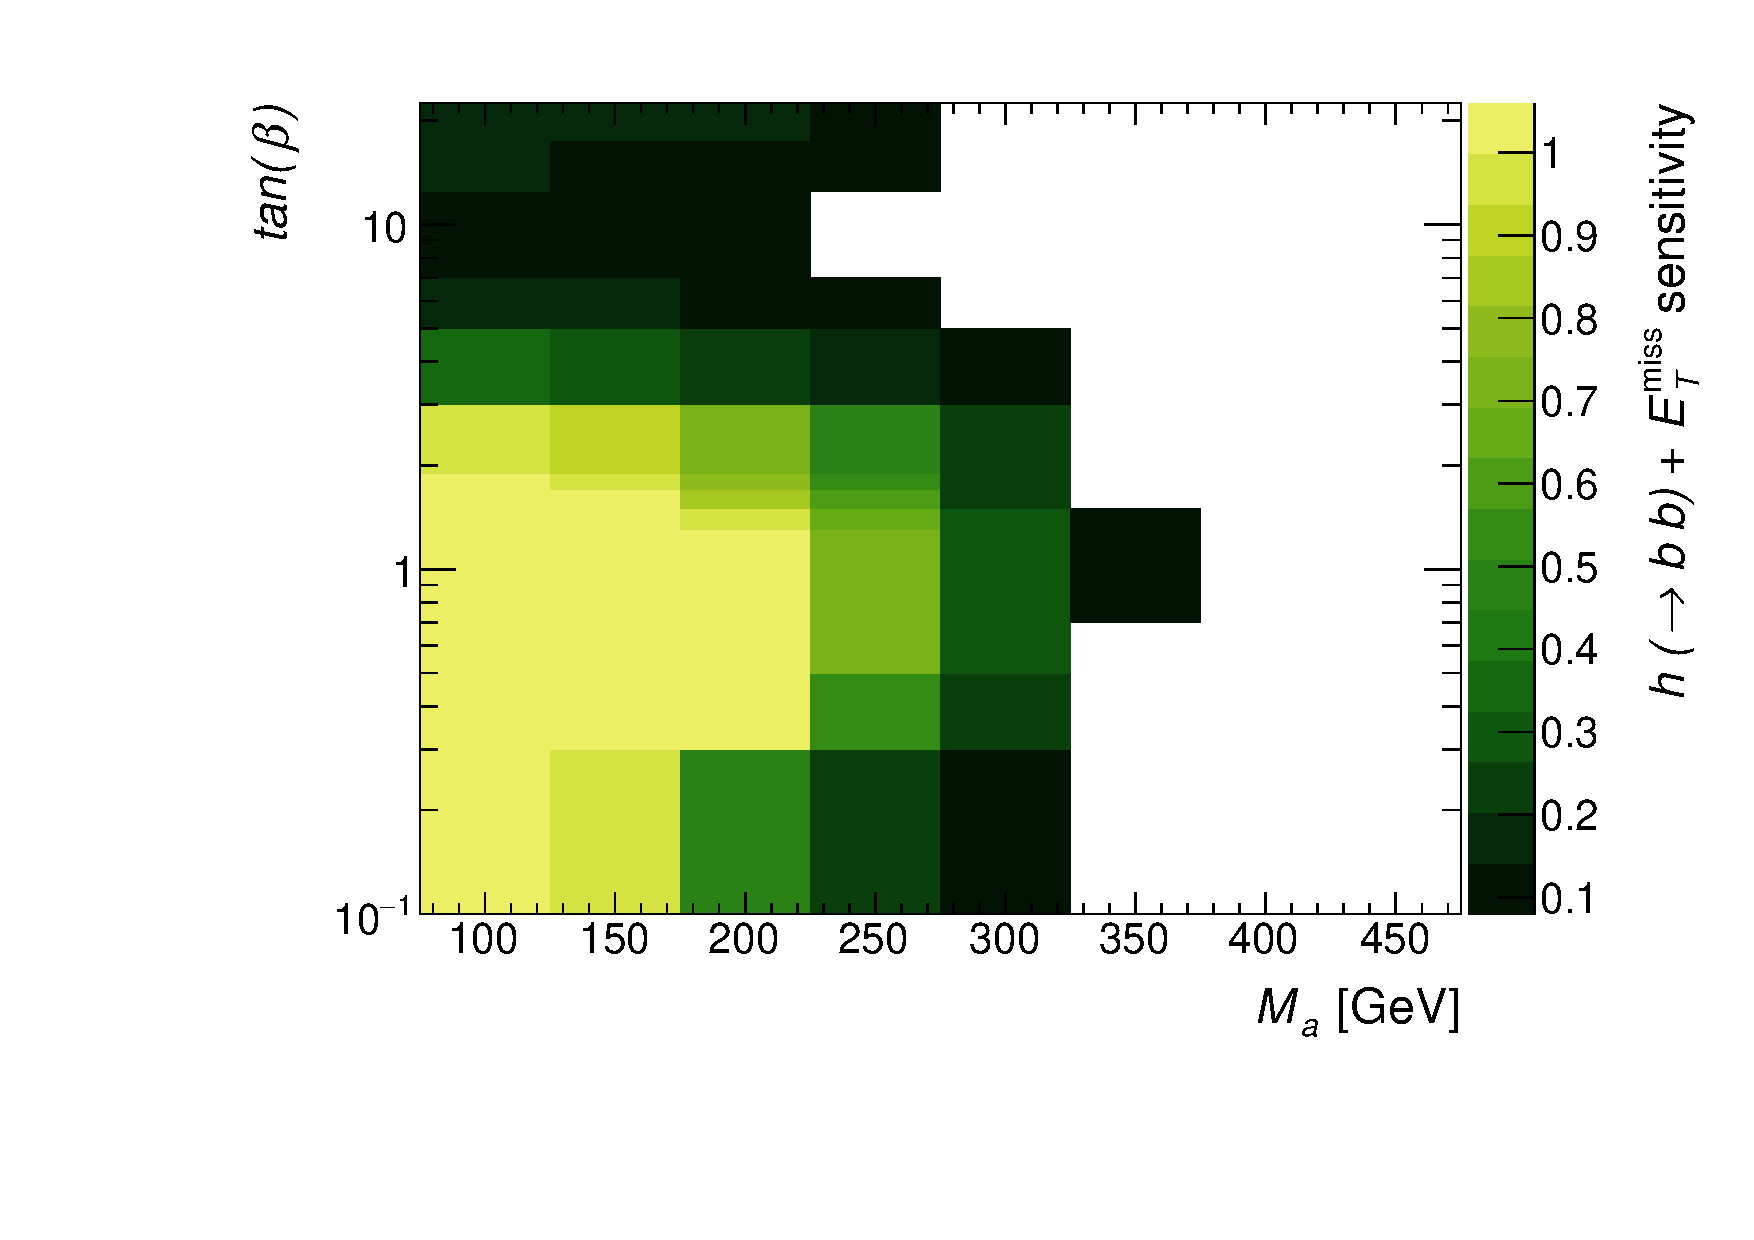
\includegraphics[width=0.75\textwidth]{texinputs/04_grid/figures/monoHbb_sensi_sum_bins_1_2_3_4_ma_vs_tanb_lin.pdf}
\vspace{2mm}
\caption{Estimated sensitivities of the $h+\MET$ signature in the $h \to b \bar b$ channel. The upper (lower) panel shows our results in the $\ma\hspace{0.25mm}$--$\hspace{0.25mm}\mA$ ($\ma\hspace{0.25mm}$--$\hspace{0.25mm}\tan \beta$) plane. {\color{red} The remaining parameters are set to \eqref{eq:benchmark} in the upper panel, while in the lower panel $\tan \beta$ is left to vary but the common 2HDM Higgs mass is fixed to~\eqref{eq:matbscan}.} Bins with no content have a negligible sensitivity. See text for further explanations. {\color{red} [Uli: Use the same notation etc. for the plots in Figures~\ref{fig:monoHbb_sensi} and \ref{fig:monoZll_sensi}!]}}
\label{fig:monoHbb_sensi}
\end{figure}

The sensitivity estimates of the ATLAS and CMS mono-Higgs searches in the $b \bar b$ channel to the \hdma model are based on the model-independent limits on the anomalous production of the SM Higgs boson in association with \met derived in~\cite{Aaboud:2017yqz}.  As these limits are set in terms of the observed production cross section of non-SM events with large $\MET$ and a Higgs boson, they can be compared directly to the cross sections obtained in the \hdma model after taking into account the kinematic acceptance $\mathcal{A}$ of the event selection and the detection efficiency $\varepsilon$. The variables of interest for the sensitivity study of the $b \bar b + \MET$ searches are 
\begin{equation}
\label{eq:monoHbb_sensi}
S_i = \frac{\sigma_{i} \left ( p p \to h + \MET \right)_{\hdma} \cdot {\rm BR} \left (h \to b \bar b \right )_{\rm SM} \cdot \left ( \mathcal{A} \cdot \varepsilon \right)_i}
{\sigma_{i} \left ( p p \to h + \MET \to b \bar b + \MET \right)_{\rm obs}}\,,
\end{equation}
where $\sigma_{i} \left ( p p \to h + \MET \right)_{\hdma}$ is the partonic cross section of the \hdma signal,  the branching ratio of the SM Higgs boson is denoted by ${\rm BR} \left (h \to b \bar b \right )_{\rm SM} \simeq 58\%$  and $\sigma_{i} \left ( p p \to h + \MET \to b \bar b + \MET \right)_{\rm obs}$ represents the  observed upper cross-section limit on $h + \MET$ production with $h \to b \bar b$. The cross sections as well as the product $ \mathcal{A} \cdot \varepsilon$ depend on the considered $\MET$ bin as indicated by the index $i$.  A particular point in parameter space is excluded if the sum $S = \sum_i S_i$ of the individual sensitivities is larger than $1$. 

The results of our sensitivity study for the mono-Higgs signal in the $b \bar b$ decay channel are shown in Figure~\ref{fig:monoHbb_sensi}. The upper panel in the figure displays $S$  as a function of $\ma$ and $\mA$. The observed cross-section limits $\sigma_{i} \left ( p p \to h + \MET \to b \bar b + \MET \right)_{\rm obs}$ as well as the products $({\cal A} \cdot  \varepsilon)_i$ that enter~\eqref{eq:monoHbb_sensi}  are  taken from the recent ATLAS study~\cite{Aaboud:2017yqz}. One observes that the existing mono-Higgs searches allow to probe/exclude \hdma scenarios with  $\mA > M_h + \ma$  and sufficiently small $\ma$ values, while they are only weakly  sensitive to models where the mass hierarchy between $A$ and $a$ is reversed,~i.e.~$\ma > M_h + \mA$. Numerically, we find that  for  a light $a$ with $\ma \simeq 100 \, {\rm GeV}$ one has $S > 1$ for all values $\mA \simeq [350, 1050] \, {\rm GeV}$. Notice that in the parameter region  $\mA > M_h + \ma$ the strong sensitivity of the search arises because the mono-Higgs signature is resonantly produced via $pp \to A \to ha \to h \chi \bar \chi$ --- see the discussion in Section~\ref{sec:resonant}. The sensitivity of the search decreases for increasing (decreasing) $M_A$ because the production rate of $pp \to A$  decreases $\big($the Jacobian peak~\eqref{eq:monoHMETpeak} is shifted to lower $\MET$ values$\big)$. In the region $\ma > M_h + \mA$, the largest contribution to the $h + \MET$ cross section again originates from resonant production, namely $pp \to a \to hA \to h \chi \bar \chi$. The resulting sensitivities are however compared to the case discussed before much smaller because  $\sigma \left (p p \to a \right )/\sigma \left (pp \to A \right ) = \sin^2 \theta/\cos^2 \theta \simeq 1/7$, ${\rm BR} \left ( a \to A h \right )/{\rm BR} \left (  A \to a h  \right ) < 1$ and ${\rm BR} \left ( A \to \chi \bar \chi \right )/{\rm BR} \left (  a \to \chi \bar \chi \right ) \ll 1$ for the parameter choices made in \eqref{eq:benchmark}. 

\begin{figure}[t!]
\centering
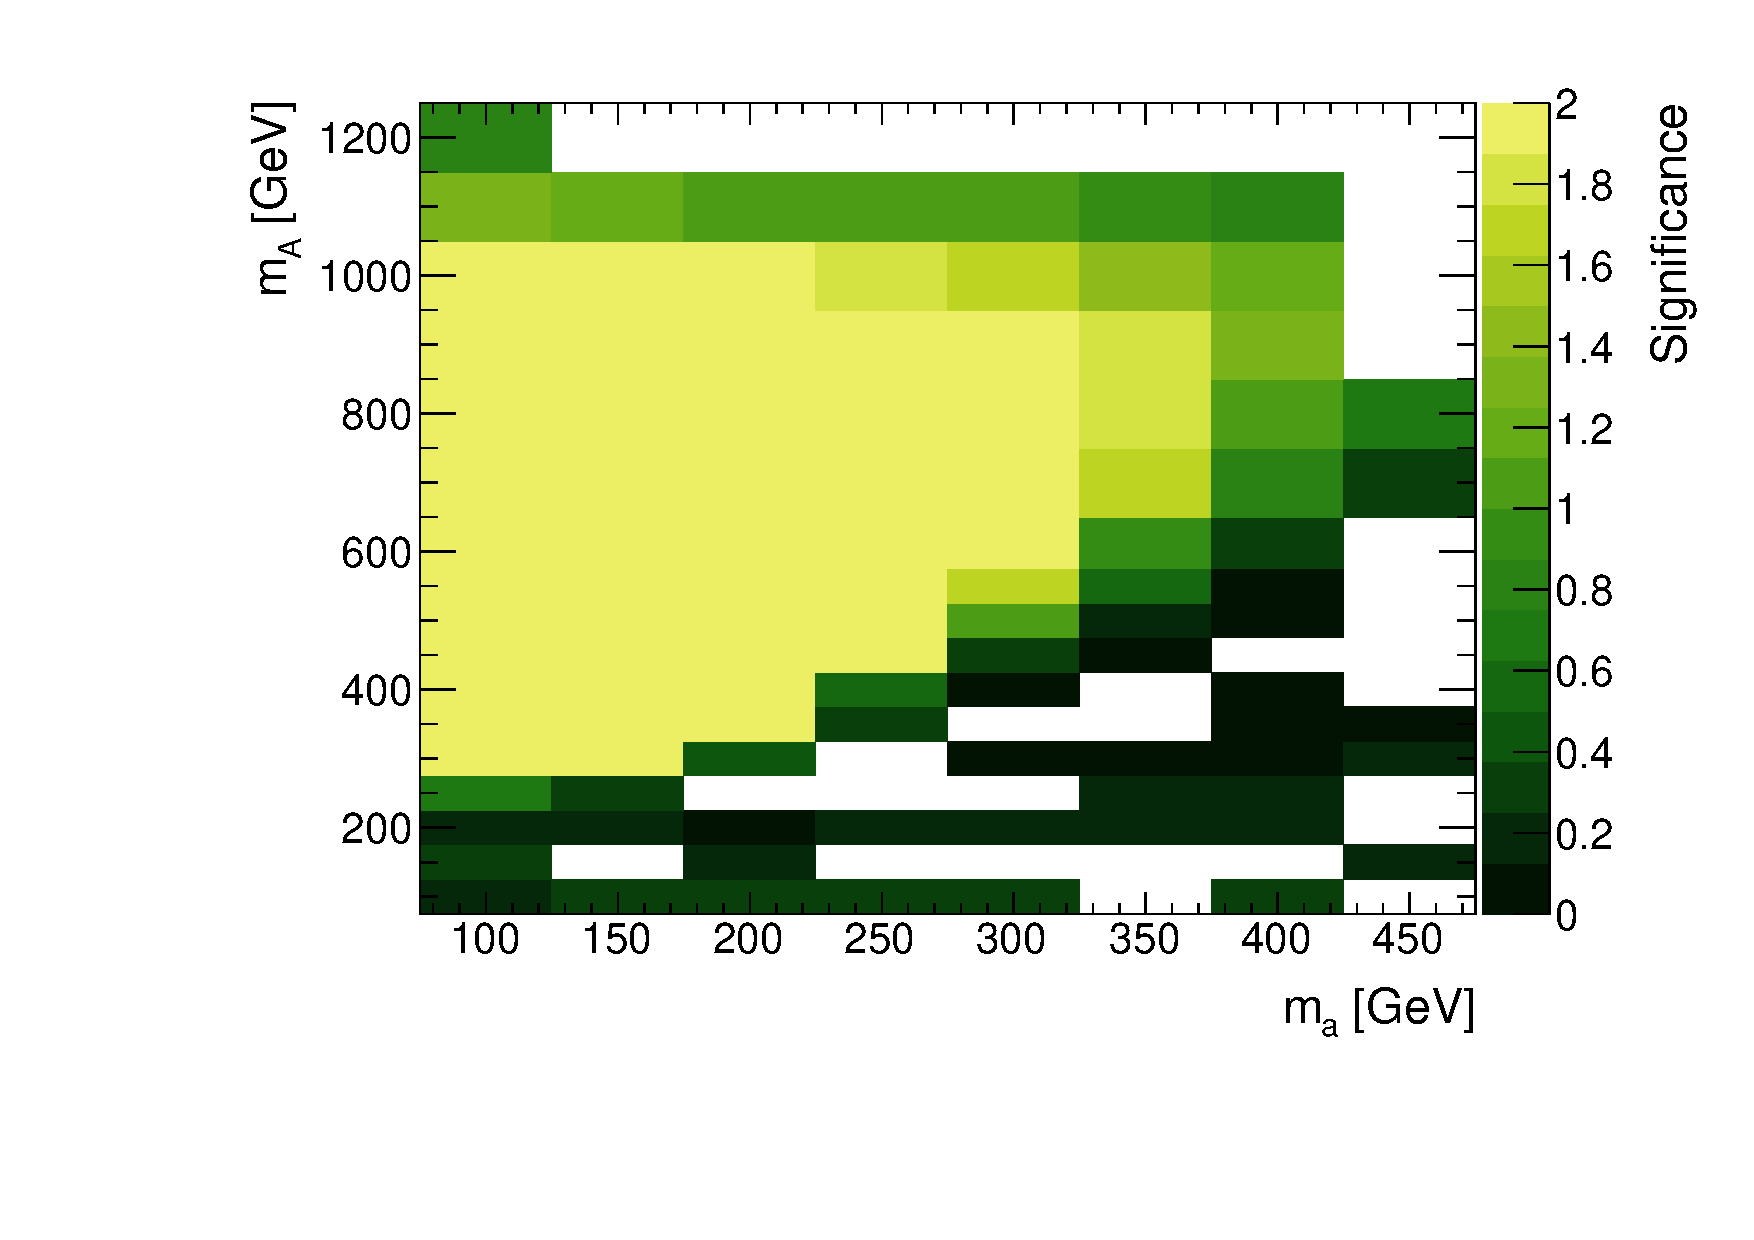
\includegraphics[width=0.75\textwidth]{texinputs/04_grid/figures/monoz/leptonic/mAma_Significance_ll.pdf}

\vspace{2mm}

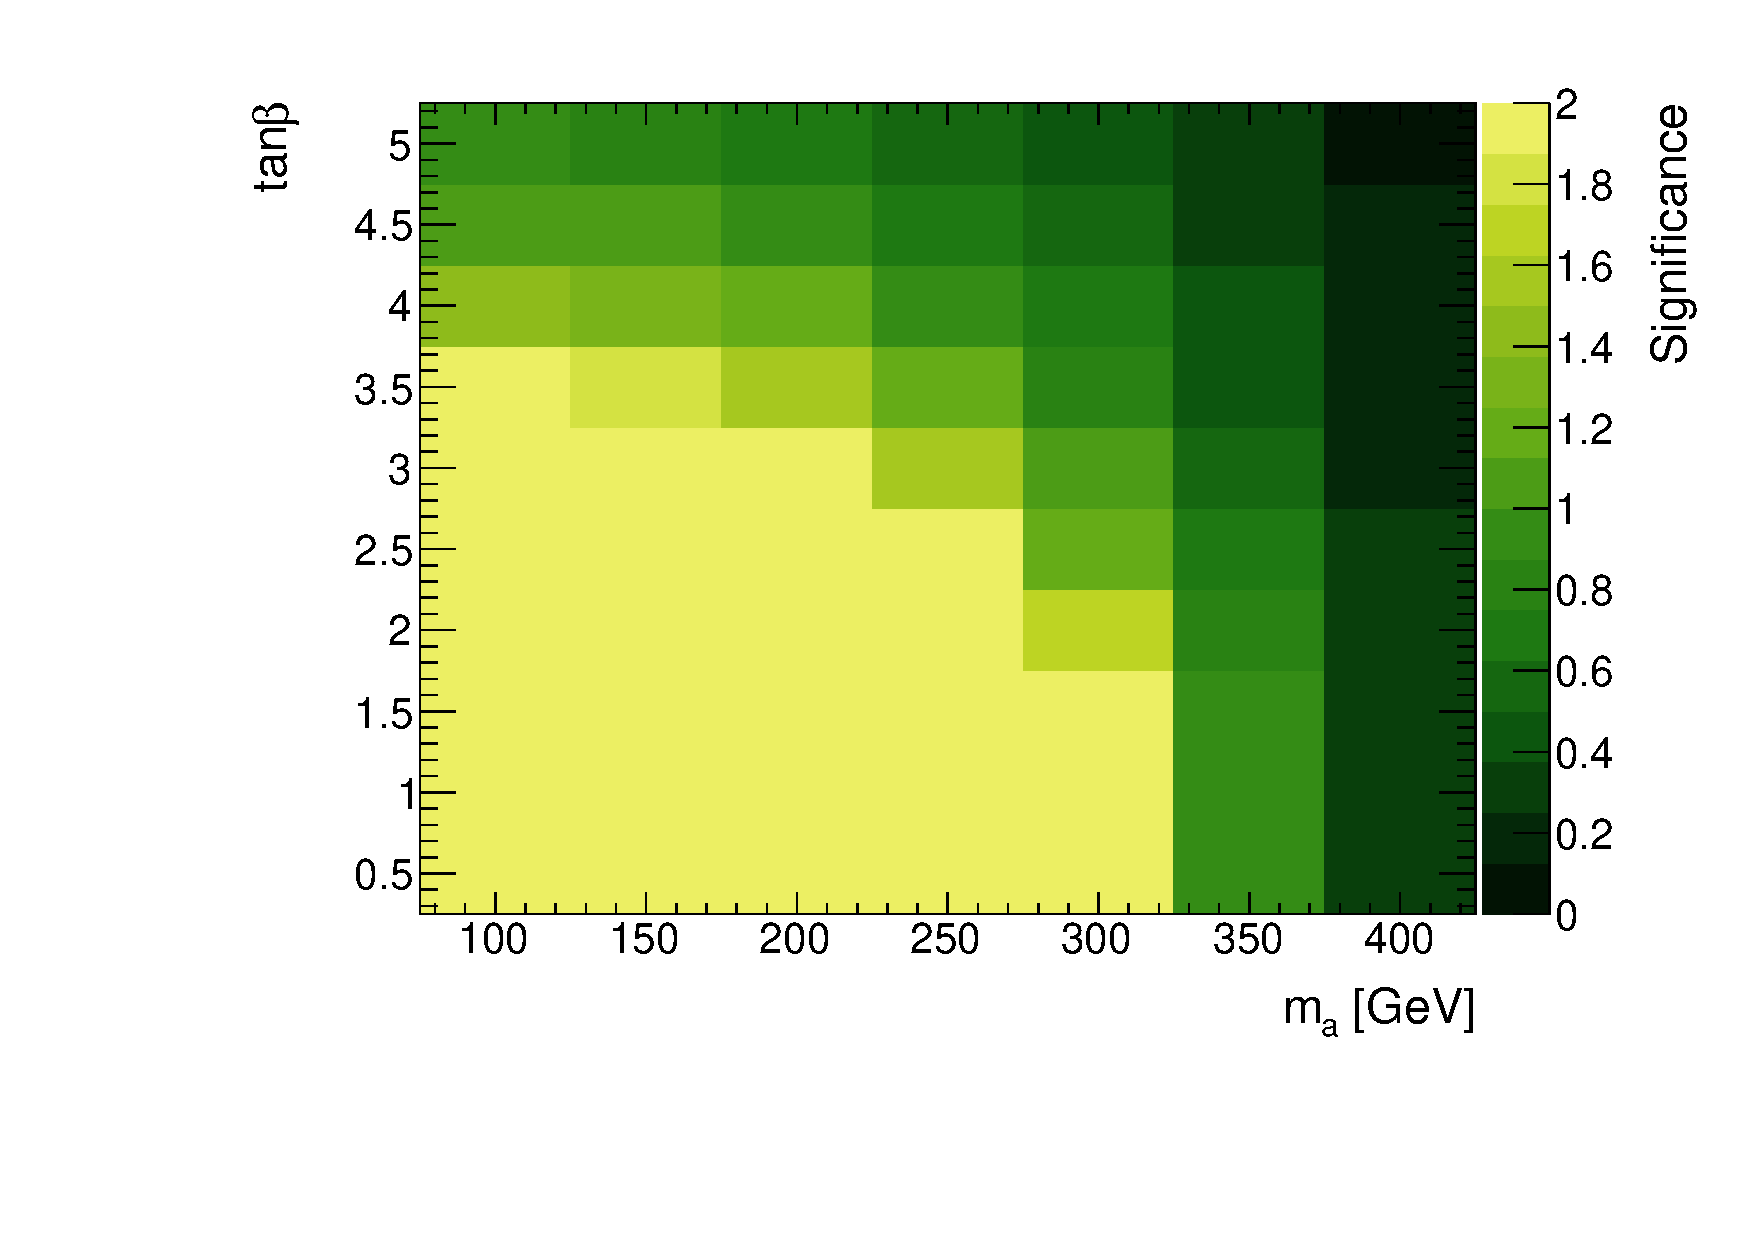
\includegraphics[width=0.75\textwidth]{texinputs/04_grid/figures/monoz/leptonic/tanbma_Significance_ll.pdf}
\vspace{2mm}
\caption{Estimated significance of the $Z+\MET$ signature in the $Z \to \ell^+ \ell^-$ channel. The upper (lower) panel shows our results in the $\ma\hspace{0.25mm}$--$\hspace{0.25mm}\mA$ ($\ma\hspace{0.25mm}$--$\hspace{0.25mm}\tan \beta$) plane. The choice of parameters resembles those made in Figure~\ref{fig:monoHbb_sensi}. Further details can be found in the text. {\color{red} [Uli: Last statement correct? In particular, choice of $\mH = \mA = \mHc$ in the case of the $\ma\hspace{0.25mm}$--$\hspace{0.25mm}\tan \beta$ plot has not been specified!] }}
\label{fig:monoZll_sensi}
\end{figure}

{\color{red} The lower panel in Figure~\ref{fig:monoHbb_sensi} shows the sensitivity $S$ in the $\ma\hspace{0.25mm}$--$\hspace{0.25mm}\tan \beta$ plane fixing  $\mH, \mA$ and  $\mHc$ to~\eqref{eq:matbscan}.} One observes that the existing mono-Higgs searches allow to exclude $\tan \beta \lesssim 3$ for $m_a \simeq 100 \, {\rm GeV}$ and $\tan \beta \lesssim 1$ for $m_a \lesssim 225 \, {\rm GeV}$. From~Figure~\ref{fig:tbvar} it is apparent that for such small values of $\tan \beta$, the $h + \MET$ signal is dominantly produced through top-quark loops in $gg$-fusion. The corresponding production rate scales as $\sigma \left ( gg \to A \right ) \propto \cot^2 \beta$, and as a result the sensitivity rapidly decreases for $\tan \beta > 1$. Notice that the decrease is to some extent counteracted by the fact that the Jacobian peak becomes more pronounced when  $\tan \beta$ is increased (cf.~the left panel in Figure~\ref{fig:tbvar}). Another feature that is visible in the  lower panel in Figure~\ref{fig:monoHbb_sensi}  is that at $\tan \beta \gtrsim 10$ the sensitivity of the mono-Higgs search  starts to increase again, because the $b \bar b$-initiated production cross section behaves like $\sigma \hspace{0.5mm} ( b \bar b \to A  ) \propto \tan^2 \beta$. Further plots of our mono-Higgs sensitivity study can be found in Appendix~\ref{app:extramonoh}.

\subsection[Mono-$Z$ study]{Mono-$\bm{Z}$ study}
\label{sec:sensi_monozll}

In the absence of model-independent limits on anomalous production of $Z + \MET$ events, the expected sensitivity of the mono-$Z$ search to the \hdma model is estimated by comparing the number of generator-level signal events to the number of expected background events. The published background predictions for $Z+\MET$ production followed by $Z \to \ell^+ \ell^-$~\cite{Aaboud:2017bja} are used which correspond to $36 \, {\rm fb}^{-1}$ of $13 \, {\rm TeV}$ data. The selection cuts and \MET binnings that are applied to the signal events resemble those employed in the ATLAS analysis~\cite{Aaboud:2017bja}. A reconstruction efficiency of 75\% is assumed for signal events,  and a conservative background systematic uncertainty of 20\% (10\%) is taken for events with $\MET < 120  \, {\rm GeV}$ ($\MET > 120  \, {\rm GeV}$). Following the Asimov approximation, the significance $Z_{A,i}$ for individual bins $i$ is calculated as a Poisson ratio of likelihoods modified to incorporate systematic uncertainties on the background. Explicitly one has \cite{Cowan:2012}
\begin{equation}
\label{eq:significance_wsyst}
Z_{A, i} = \sqrt{ 2 \left ( \left ( s + b \right ) \ln \left [ \frac{\left (s+b \right ) \left (b + \sigma_b^2 \right )}{b^2 + \left ( s +b \right ) \sigma_b^2 } \right ]  - \frac{b^2}{\sigma_b^2} \ln \left [ 1 + \frac{\sigma_b^2 s}{b \left ( b + \sigma_b^2 \right )} \right ] \right ) } \,, 
\end{equation}
where $s$ ($b$) represents the expected number of signal (background) events and $\sigma_s$ ($ \sigma_b$) denotes the corresponding standard deviation that characterises systematic uncertainties. The total significance $Z_A$ is then defined by adding the individual $Z_{A, i}$ in quadrature. The ATLAS and CMS experiments are expected to be sensitive to regions with total significances of~$Z_A > 2$. %{\color{red} [Uli: Why $Z_A > 2$? Since $Z_A = \Phi^{-1} (1 - p)$ with $\Phi^{-1}$ the quantile of the standard Gaussian distribution, a 95\% CL corresponds to $Z_A = 1.64$. $Z_A = 2$ corresponds to around 98\% CL. What is the connection to the CLs method?]}
 
The results of our sensitivity study for the mono-$Z$ signature in the $\ell^+ \ell^-$ channel are presented in Figure~\ref{fig:monoZll_sensi}. The upper (lower) panel displays the total significance $Z_A$  in the $\ma\hspace{0.25mm}$--$\hspace{0.25mm}\mA$ ($\ma\hspace{0.25mm}$--$\hspace{0.25mm}\tan \beta$) plane. Comparing the obtained results to those depicted in Figure~\ref{fig:monoHbb_sensi}, one observes that for the parameter choices~\eqref{eq:benchmark} the mono-$Z$ and mono-Higgs searches allow to test quite similar parameter regions in the $\ma\hspace{0.25mm}$--$\hspace{0.25mm}\mA$ plane. Numerically, we find  that for $\ma \simeq 100 \, {\rm GeV}$  the existing $Z + \MET$ searches are sensitive to 2HDM pseudoscalar masses  in the range of $\mA \simeq [300, 1050] \, {\rm GeV}$. Notice that the mono-$Z$ sensitivity to lower values of $M_A$ is slightly better than the one found in the mono-Higgs case. This enhanced sensitivity arises because for fixed $M_A$ and $M_a$ and given that $M_Z < M_h$ the endpoint $E_{T, \rm max}^{\rm miss}$ of the $\MET$ distribution in $Z+ \MET$ production is always higher  than that in  the $h+ \MET$ channel. In contrast, in the parameter region with $M_a > M_Z + M_A$ the sensitivity of the mono-$Z$ signature is weaker than that of the mono-Higgs  signal. This feature is readily understood by noticing that the $pp \to a \to Z H$ channel does not lead to a $\MET$ signature, since the scalar $H$ does not decay invisibly in the \hdma model. For $M_a > M_Z + M_A$ hence only non-resonant diagrams contribute to the $Z+\MET$ signature, and the sensitivity to such model realisations is consequently very weak. 

{\color{red} In the lower panel of Figure~\ref{fig:monoZll_sensi} we plot the significance $Z_A$ in the $\ma\hspace{0.25mm}$--$\hspace{0.25mm}\tan \beta$ plane for the choice~\eqref{eq:matbscan}. } {\color{red} [Uli: Correct? Or other choice?]} We see that present mono-$Z$ searches are able to exclude $\tan \beta \lesssim 3.5$ for $m_a \simeq 100 \, {\rm GeV}$ and $\tan \beta \lesssim 1$ for $m_a \lesssim 325 \, {\rm GeV}$. The quoted exclusion limits compare favourable with the mono-Higgs case. We add that in models where the bottom-quark Yukawa coupling is $\tan \beta$ enhanced such as the type-II scenario studied here, $b \bar b \to Z + \MET$ production starts to become relevant for  $\tan \beta \gtrsim 10$~\cite{Bauer:2017ota}. Since only $gg$-fusion but not $b \bar b$-fusion production is included in our mono-$Z$ simulations, only $\tan \beta$ values up to 5.5 are plotted in the lower panel of Figure~\ref{fig:monoZll_sensi}. Further details on our mono-$Z$ sensitivity study are given in Appendix~\ref{app:extramonoz}.

\subsection[Sensitivity of other mono-$X$ channels]{Sensitivity of other mono-$\bm{X}$ channels}
\label{sec:sensi_others}

The sensitivities of the LHC to the associated production of DM with a single top has been  studied in the framework of the \hdma model in~\cite{Pani:2017qyd}. This analysis assumes $300 \, {\rm fb}^{-1}$ of data and finds that the $t X + \MET$ signatures complement the parameter space coverage of the mono-Higgs and  mono-$Z$ signals considered by us in detail.  Since searches for associated production of DM with a single top have so far not been performed at the LHC, one cannot use existing model-independent limits to estimate the sensitivity of these channels. For this reason we do not perform a sensitivity study of the $t X + \MET$ signatures in this whitepaper. 

Sensitivity studies of the $t \bar t + \MET$ and $j + \MET$ channels in the \hdma have been performed in~\cite{Bauer:2017ota}. The results presented in that work imply that for the benchmark parameter choices~\eqref{eq:benchmark}, the latest  $t \bar t + \MET$ and  mono-jet searches that are based on $36 \, {\rm fb}^{-1}$ of 13 TeV data have  only a very weak sensitivity to the parameter space shown in Figures~\ref{fig:monoHbb_sensi} and \ref{fig:monoZll_sensi}. Given the weak sensitivity of the $t \bar t + \MET$ and $j + \MET$ modes we do not perform sensitivity studies for these channels in this whitepaper. The $b \bar b + \MET$ channel is also not considered here due to the same reason. Notice however that a reinterpretion of existing $t \bar t + \MET$, $b \bar b + \MET$ and $j + \MET$ results is straightforward by using the general rescaling strategy discussed in Appendix~\ref{app:recast}. 










